\chapter{Verifikation durch Coq}
\label{ch:coq}
Die Theorie des Teilformelkalküls und der Teilformelfiltration, die in dem letzten Kapitel vorgestellt wurden, wurde im Rahmen dieser Arbeit formalisiert und in Teilen mit einem computergestützten Beweishelfer verifiziert. Als System wurde hier \coq{}\footnote{\url{https://coq.inria.fr/}} in der Version 8.8.0 gewählt. Die hier vorgestellte Implementierung liegt einerseits der Arbeit bei und lässt sich unter \url{https://github.com/christofsteel/PrincInh/} abrufen. Diese Arbeit bezieht sich auf den Tag \texttt{final} (Commit \texttt{e1bdae8}). Die Implementierung steht unter der \emph{Apache-2.0-Lizenz}\footnote{\url{https://opensource.org/licenses/Apache-2.0}}. 

Wir werden zunächst den Aufbau der grundlegenden Datentypen sowie den wichtigsten Lemmata zu diesen betrachten, um darauf aufbauend die Verifikation für \Cref{lem:filtrprinc} der Teilformelfiltration und \Cref{lem:fz} des Teilformelkalküls zu untersuchen.
\section{Aufbau der Implementierung}
\begin{table}
    \begin{center}
        \begin{tabular}{l|p{10.5cm}}
            \textbf{Datei} & \textbf{Beschreibung}\\
            \hline
            \hline
            \texttt{Utils.v} & Grundlegende Hilfsfunktionen und Konstruktionen.\\
            \texttt{Terms.v} & Definition von $\lambda$-Termen.\\
            \texttt{Terms2.v} & Alternative Definition von $\lambda$-Termen.\\            
            \texttt{NFTerms.v} & Alternative Definition von \tlambda-Termen in \tbeta-Normalform.\\        
            \texttt{Types.v} & Definition der einfachen Typen.\\
            \texttt{Typing.v} & Definition der Typableitung für einfache Typen, Terme und NFTerme.\\
            \texttt{LongTyping.v} & Definition der Langableitung.\\        
            \texttt{Filtr.v} & Teilformelfiltration und Implementierung von \Cref{lem:filtrprinc}.\\
            \texttt{Paths.v} & Definition von und Aussagen über Pfade in Termen.\\
            \texttt{SfC.v} & Verifikation des Teilformelkalküls bis einschließlich \Cref{lem:fz}, sowie Stubs zu den folgenden Lemmata.\\                        
        \end{tabular}
    \end{center}
\caption{Übersicht der Quelltextdateien}
\label{tab:impl}
\end{table}
Der grundlegende Aufbau der Implementierung ist über \Cref{tab:impl} gegeben. Als externe Bibliothek wurde lediglich \textsc{Autosubst} verwendet \cite{autosubst}. \textsc{Autosubst} stellt Klassen bereit, über die Substitutionen definiert sind und generiert Lemmata, die den Umgang mit diesen Substitutionen vereinfachen. Da wir hier hauptsächlich Terme betrachten, die bereits in $\beta$-Normalform vorliegen, wurde dieser Teil nicht intensiv genutzt.

In den folgenden Abschnitten werden wir viele Listings betrachten; diese sind -- falls vorhanden -- immer mit der entsprechenden Quelltextdatei sowie der entsprechenden Zeilennummer annotiert. Der Quelltext musste an einigen Stellen für das Einbetten in diese Arbeit verändert werden. Dies betrifft jedoch lediglich Formatierungen. Dennoch können dadurch einige Zeilennummern nicht mehr mit den Zeilennummern im Originalquelltext übereinstimmen. Die Zeilennummer der ersten Zeile ist jedoch in jedem Fall korrekt. Die Implementierungen von Lemmata werden an dieser Stelle nicht angegeben, sondern in den wichtigsten Fällen beschrieben. Lediglich der Typ der Lemmata, also die Aussage der Lemmata, wird hier abgedruckt. Konstruktionen und Funktionen werden jedoch explizit angegeben und diskutiert.

\section{\Type, \Prop{} und \Set}
\coq{} ist eine Sprache mit \emph{higher order dependent typing}. Wir werden auf die genaue Theorie hinter \coq{} nicht im Detail eingehen, jedoch flossen einige Eigenschaften \coq s in Designentscheidungen der Formalisierung ein, die hier kurz erörtert werden.

Der Begriff \emph{higher order dependent typing} bedeutet im Kern, dass wir sowohl Typen als Objekte betrachten können, die ihrerseits wieder Typen haben können (\emph{higher order}), sowie, dass wir Objekte als Typen nutzen können, sodass ein Typ abhängig von dem Wert eines Objektes sein kann (\emph{dependent typing}). Die Zahl $2$ ist somit ein gültiger Typ und der Datentyp \texttt{nat} der natürlichen Zahlen ist ein gültiges Objekt, das einen eigenen Typen hat.
  
Der allgemeinste Typ, den \coq{} kennt, ist \Type{}. Er agiert als Metatyp für Datentypen, die in \coq{} aufgestellt und genutzt werden. Weitere allgemeine Typen, die in \coq{} als Metatypen genutzt werden, sind \Prop{} und \Set. Da \Type{} der allgemeinste Typ ist, gilt $\Prop\prec\Type$ und $\Set\prec\Type$, und \Prop{}, \Set{} und \Type{} haben jeweils den Typen \Type. 
\begin{figure}[t]
    \begin{center}
        \begin{tikzpicture}[node distance=1.5cm]
        \node (T0) at (0,0) {$\Type_0$};    
        \node (T1) [above of= T0] {$\Type_1$};
        \node (dots) [above of = T1] {$\vdots$};
        \node (P) [below left of = T0] {\Prop};
        \node (S) [below right of = T0] {\Set};
        \draw (T1) -- (T0);
        \draw (T1) -- (dots);
        \draw (T0) -- (P);
        \draw (T0) -- (S);
        \end{tikzpicture}
    \end{center}
    \caption{Hierarchie von \Type, \Prop{} und \Set}
    \label{fig:TypePropSet}
\end{figure}
\begin{icode}
    \QA{Check Prop.}{Prop : Type}
    \QA{Check Set.}{Set : Type}
    \QA{Check Type.}{Type : Type}        
\end{icode}

Dies führt dazu, dass \Type{} sich selbst typt und über \emph{Girards Paradox} dazu, dass das Typsystem von \coq{} inkonsistent wäre\cite{Coquand86ananalysis}. Dieses Problem wird in \coq{} dadurch umgangen, dass es eine Hierarchie an \Type-Typen gibt. Jeder Typ \Type{} der Ebene $n$ wird von einem Typ \Type{} der Ebene $n + 1$ getypt. Des Weiteren gilt $\Type_n \prec \Type_{n+1}$. Siehe hierzu \Cref{fig:TypePropSet}. In \coq{} wird diese Hierarchie Universum genannt und üblicherweise vor dem Anwender versteckt. 

Für Datentypen wird in \coq{} üblicherweise der Typ \Set{} verwendet. So hat Beispielsweise der Typ der natürlichen Zahlen \texttt{nat} den Typen \Set.
\begin{icode}
    \QA{Check nat.}{nat : Set}
\end{icode} 
    
Über den \emph{Curry-Howard-Isomorphismus} wissen wir, dass wir Aussagen als Typen auffassen können und Beweise als $\lambda$-Terme, die diesen Typen inhabitieren\footnote{Siehe \Cref{sec:IPC}.}. Das Typsystem von \coq{} ist deutlich mächtiger als der einfach getypte Lambda-Kalkül und entspricht somit auch einer deutlich ausdrucksstärkeren Logik als dem implikativen Fragment der intuitionistischen Logik. Für Aussagen, die in \coq{} formalisiert werden, wird üblicherweise der Typ \Prop{} verwendet.
\begin{icode}
    \QA{Check 3 < 7.}{3 < 7 : Prop}
\end{icode}

Während \Type, \Prop{} und \Set{} als allgemeine Typen ähnlich verwendet werden können, ergeben sich Probleme, wenn in sie in Konstruktionen gemischt werden.
Der Unterschied in der Behandlung von \Set{} und \Prop{} liegt darin, dass \coq{} für Typen in \Set{} Inhabitanten voneinander unterscheidet, für Typen in \Prop{} jedoch nicht. Es ist klar, dass wir zwischen zwei natürlichen Zahlen unterscheiden wollen, aber für Aussagen ist es für uns üblicherweise nur von Interesse, ob sie gelten, oder nicht, also ob ihr Typ inhabitiert wird, oder nicht. Diese Art von Beweisirrelevanz wird genutzt, wenn aus \coq{} verifizierte Programme exportiert werden.
 
Wenn wir nun die Existenz eines Inhabitanten für einen Typen in \Prop{} beweisen wollen, können wir dafür Fallunterscheidungen über Beweise zu Aussagen in \Prop{} treffen. Da der äußere Beweis nicht mitexportiert wird, muss auch der innere Beweis nicht exportiert werden. Wenn wir jedoch einen Inhabitanten eines Typen in \Set{} aufstellen wollen, können wir dafür Inhabitanten von Typen in \Prop{} nicht auseinandernehmen, da im Export dieser Teil des Inhabitantens fehlen würde.

Ein Problem ergibt sich insbesondere aus existentiell quantifizierte Aussagen sowie Disjunktionen. Eine Aussage der Form $\exists x.\varphi$, sowie $\psi\lor\varphi$ kann mehrere verschiedene Beweise haben. Der korrespondierende Typ kann somit mehrere verschiedene Inhabitanten haben. In \coq{} ist der resultierende Typ beider Konstruktionen in \Prop{}. Somit kann für Beweise in \Set{} die Konstruktion nicht auseinandergenommen werden. Für Konstruktionen in \Set{} werden stattdessen \texttt{sumbool} und \texttt{sigT} verwendet. Anstelle \icoq{A \/ B : Prop} kann \icoq{{A} + {B} : Set} und anstelle \icoq{exists x, A. P : Prop} kann \icoq{{x : A & P} : Type} verwendet werden.

Betrachten wir die Definition der relevanten Typen in \Cref{def:TD}. Das Enthaltensein in der Menge $T(\mathcal{D})$ wird über eine Eigenschaft aus $\mathcal{D}$ bestimmt. Da wir die verschiedene Elemente der Menge unterscheiden wollen, eignet sich für $T(\mathcal{D})$ eine Konstruktion in \Set. Dadurch können wir die Typableitung, über die $\mathcal{D}$ definiert ist, nicht in \Prop{} definieren. Aus diesem Grund wählen wir \Type{} als Metatyp für unsere Konstruktionen und damit auch für unsere Aussagen, da \Type{} sowohl ein Supertyp von \Set{} als auch ein Supertyp von \Prop{} ist. Dies erlaubt es uns, an einigen Stellen Lemmata der Standardbibliothek zu nutzen, die für \Prop{} definiert sind, aber gleichzeitig in Beweisen und Konstruktionen $\mathcal{D}$ auseinanderzunehmen. Zwar können so viele Lemmata, die Aussagen über Typen in $\Prop$ treffen weiterverwendet werden; Konstruktionen, die für $\Prop$ definiert wurden und in eigenen Typen verwendet werden, mussten jedoch in $\Type$ neu implementiert werden. Diese Neuimplementierungen, sowie entsprechende Lemmata zu diesen, finden sich zum Großteil in der Datei \texttt{Utils.v}.

\section{Datentypen}

Wir betrachten zunächst die grundlegenden Datentypen, die wir zur Formalisierung des einfach getypten Lambda-Kalküls benötigen, also \tlambda-Terme und einfache Typen, wobei für erstere verschiedene Definitionen aufgestellt werden. Anschließend werden Typ- und die Langableitung auf den jeweiligen Termmodellen definiert.

\subsection{\tlambda-Terme}
Anstelle der \tlambda-Terme, wie sie in \Cref{def:preterm,def:term} definiert sind, nutzen wir Terme in \emph{De-Bruijn-Notation}, gemäß \Cref{def:debruijn}.

\begin{code}[term]{Terms.v}{Siehe \Cref{def:debruijn}}{16}
Inductive term :=
  | Var (x : var)
  | App (p q : term)
  | Lam (s : {bind term}).
\end{code}

\begin{remark}
    Der Datentyp \texttt{var} ist nur ein anderer Name für \texttt{nat}.
\end{remark}

Betrachten wir den Konstruktor \texttt{Lam} in \Cref{lst:term}, so stellen wir fest, dass der Parameter nicht nur vom Typ \coqrefnl{term} ist, sondern vom Typ \texttt{{bind term}}. Dies annotiert den inneren Term mit seiner Bindungstiefe und wird von \textsc{Autosubst} intern benutzt. Wir können dies an dieser Stelle ignorieren und \texttt{s} wie einen regulären Term behandeln. 

Anstelle die Konstruktoren des Datentyps direkt zu nutzen, nutzen wir \coq s Möglichkeit, kompaktere Notationen zu definieren.

\begin{ccode}[termnot]{Terms.v}{}{22}{Notation für \texttt{term}}
Notation "'!' x" := (Var x) (at level 15).
Notation "p '@' q" := (App p q) 
    (at level 31, left associativity).
Notation "'\_' p" := (Lam p) (at level 35, right associativity).     
\end{ccode}

Die Terme \tI, \tK{} und \tS{} lassen sich nun folgendermaßen in \Cref{lst:SKI} darstellen.
\begin{ccode}[SKI]{Terms.v}{Siehe \Cref{ex:debruijn}}{31}{\texttt{tI}, \texttt{tK} und \texttt{tS}}
Definition tI := \_ !0.
Definition tK := \_ \_ !0.
Definition tS := \_\_\_((!2@!0)@(!1@!0)).
\end{ccode}

\textsc{Autosubst} definiert Klassen, über denen Substitutionen definiert sind. Mittels der Taktik \texttt{derive} können, sofern der entsprechende Datentyp nicht zu komplex ist und mittels \texttt{var} und \texttt{bind} definiert ist, automatisch diese Klassen erfüllt werden. Die Instanziierung der Klassen ist in \Cref{lst:terminst} zu sehen.

\begin{ccode}[terminst]{Terms.v}{}{26}{Autosubstinstanzen für \texttt{term}}
Instance Ids_term : Ids term. derive. Defined.
Instance Rename_term : Rename term. derive. Defined.
Instance Subst_term : Subst term. derive. Defined.
Instance SubstLemmas_term : SubstLemmas term. derive. Qed.
\end{ccode}

Über die Klasse \texttt{Subst} ist die Substitutionsfunktion \texttt{subst} definiert, die eine 
Variablensubstitutionsfunktion auf Terme fortsetzt. 
\begin{icode}
    \QA{Check subst.}{subst : (var -> term) -> term -> term}
\end{icode}
Dies entspricht unserer Substitution gemäß \Cref{def:subst}.
Auf dieser Basis kann nun in \Cref{lst:step} die \tbeta-Reduktion implementiert werden.
\begin{code}[step]{Terms.v}{Siehe \Cref{def:betared}}{73}
Inductive step : term -> term -> Prop :=
  | Step_beta (s1 s2 t : term) :
      s1.[t/] = s2 -> step (App (Lam s1) t) s2
  | Step_appL (s1 s2 t : term) :
      step s1 s2 -> step (App s1 t) (App s2 t)
  | Step_appR (s t1 t2 : term) :
      step t1 t2 -> step (App s t1) (App s t2)
  | Step_lam (s1 s2 : term) :
      step s1 s2 -> step (Lam s1) (Lam s2).
\end{code}
\begin{remark}
    \texttt{s1.[t/]} entspricht \texttt{subst (t .: ids) s1}. Die Funktion \icoq{ids : var -> term} ist über die Klasse \texttt{Ids} definiert und entspricht einer Substitution, die einer Variablen \texttt{n} ihren den Term \texttt{! n} zuweist. Wird diese auf Terme geliftet, entspricht dies der Identität. Der Operator \texttt{.:} entspricht der Funktion \icoq{scons (m : term) (Su : var -> term): var -> term} und verschiebt die Zuweisungen einer übergebenden Funktion \texttt{Su} um $1$ und überschreibt die erste Position mit \texttt{m}. 
    
    Eine Substitution wird im Grunde über die Funktion aus den natürlichen Zahlen als unendliche Liste interpretiert, die für jede Variable -- also natürliche Zahl -- einen Wert hat.
    
    Da in der Reduktion eine Abstraktion entfernt wird, sinkt der Abstand aller inneren Variablen zu ihrer entsprechenden Abstraktion um $1$. Dies wird mit dem Verschieben um $1$ gelöst und die ehemalige Variable $0$ entspricht genau der Variable, die durch die Reduktion ersetzt wird.
\end{remark}

Über die Reduktion lässt sich nun der Begriff der \tbeta-Normalform in \Cref{lst:NF} definieren.
\begin{code}[NF]{Terms.v}{}{143}
Definition NF (t : term) := forall t', ¬step t t'.
\end{code}

\subsubsection{Terme mit zwei Konstruktoren}

Betrachten wir \Cref{def:longtype,def:SfC}, so stellen wir fest, dass die Ableitungsregeln im Gegensatz zu denen aus \Cref{def:typing} auf Basis von zwei, anstelle von drei Konstruktoren definiert sind. 

Eine Möglichkeit, \tlambda-Terme auf Basis von zwei Konstruktoren zu definieren, ist es, die Terme grundsätzlich als Liste von Applikationen zu sehen. Wir haben nun entweder eine Variable oder eine Abstraktion, auf die jeweils eine Liste von Termen angewendet wird.
\Cref{lst:term2} zeigt die Implementierung solcher Terme.
\begin{code}[term2]{Terms2.v}{}{9}
Inductive term2 :=
  | App_var (ms : list term2) (x : var)
  | App_lam (ms : list term2) (s : {bind term2}).
\end{code}
\begin{remark}
    Die Konstruktoren erwarten zunächst eine Liste von Termen und anschließend eine Variable oder eine Abstraktion. Dies vereinfacht \textsc{Autosubst} die Generierung von Substitutionslemmata.
\end{remark}

Auch hier können wir eine Notation einführen. Dies ist in \Cref{lst:term2not} zu sehen.
\begin{ccode}[term2not]{Term2.v}{}{37}{Notation für \texttt{term2}}
Notation "'!!!' x" := (App_var [] x) (at level 15).
Notation "'!!' p '@@' q" := (App_var q p) 
  (at level 31, left associativity).
Notation "'\___' p" := (App_lam [] p) 
  (at level 35, right associativity). 
Notation "'\__' p '@@' q" := (App_lam q p) 
  (at level 35, right associativity). 
\end{ccode}    

Die Datei \texttt{Terms2.v} enthält die Implementierung für diese Art von Terme, inklusive der folgenden Funktionen, die beide \tlambda-Termvarianten ineinander überführen, sowie Lemmata, die zeigen, dass beide Definitionen isomorph zueinander sind und einigen weiteren Lemmata und Konstruktionen, die es erlauben, Substitutionen auf den Termen durchzuführen. Diese sind in \Cref{lst:term2term} gelistet, hierbei ist \icoq{>>>} die Funktionskomposition.
 
\begin{multicode}[term2term]{Terms2.v}{}{\texttt{term2\_term}, \texttt{term\_term2}, \texttt{term2\_term\_id}, \texttt{term\_term2\_id}, \texttt{term2\_term\_if} und \texttt{term\_term2\_if}}
    \begin{mcode}{43}
Fixpoint term2_term (m : term2) : term
    \end{mcode}
    \begin{mcode}{49}
Fixpoint term_term2 (m : term) : term2
\end{mcode}    
\begin{mcode}{60}
Lemma term2_term_id : forall m, (term2_term >>> term_term2) m = m.
\end{mcode}
\begin{mcode}{88}
Lemma term_term2_id : forall m, (term_term2 >>> term2_term) m = m.
\end{mcode}
\begin{mcode}{101}
Lemma term2_term_if : forall m n, 
    term2_term m = term2_term n -> m = n.
\end{mcode}
\begin{mcode}{111}
Lemma term_term2_if : forall m n, 
    term_term2 m = term_term2 n -> m = n.
\end{mcode}
\end{multicode}

Die Konstruktion aus \texttt{Term2.v} erlaubt es uns für die (long) und (varapp)$_R$ Regel die Konstruktion \icoq{!! x @@ [m_1;...;m_n]} und für die (abs) und (abs)$_R$ die Notation \icoq{\___ m} zu verwenden.
Im Fall der Abstraktion können wir jedoch beobachten, dass sowohl für die Lang-, als auch für die Pfadableitung, keine Terme der Form \icoq{\__ s @@ [m_1, ... ,m_n]} benutzt werden. Die in \texttt{Term2.v} definierten Terme haben zwar genau zwei Konstruktoren und sind isomorph zu den in \texttt{Term.v} definierten Termen, passen aber immer noch nicht genau auf die Terme, die in der Langableitung und dem Teilformelkalkül erwartet werden. Aus diesem Grund werden wir diese Terme in unserer weiteren Implementierung nicht nutzen. Sie stellen jedoch einen wichtigen Schritt für die folgende Implementierung von \tlambda-Termen dar.

\subsubsection{Terme in Normalform}
Wenn wir nun verbieten, dass Abstraktionen als erstes Element einer Applikation vorkommen, erhalten wir eine Art von \tlambda-Termen, deren Konstruktoren genau auf die Lang- und Pfadableitung passen, die in \Cref{lst:nfterm} präsentiert wird.
\begin{code}[nfterm]{NFTerms.v}{}{11}
Inductive nfterm :=
  | NFcurr (ms: list nfterm) (x : var)
  | NFLam (s: {bind nfterm}).
\end{code}

Es fällt auf, dass mit dieser Definition der \tlambda-Terme, nicht alle Terme abgebildet werden können. Grundsätzlich können wir keine Terme darstellen, die Redexe haben (siehe \Cref{def:redex}). Daraus folgt, dass wir nur Terme darstellen können die in \tbeta-Normalform sind. Dies stellt sich jedoch als kein Problem heraus, da wir uns weitestgehend auf Terme in $\eta$-langer Normalform beschränken. Die in \texttt{NFTerms.v} definierten Funktionen \icoq{NFterm_term (nft : nfterm) : term} und \icoq{term_NFterm (t : term) : option term} bilden von den regulären \tlambda-Termen in die NFTerme ab. Dies erlaubt es uns Resultate über den Termen, die in diesem Abschnitt definiert werden, auf die regulären \tlambda-Terme zu übertragen. %Die Lemmata \icoq{NFterm_term_inv1 : forall t, term_NFterm (NFterm_term t) = Some t} und \icoq{}

Da die Terme aus \texttt{Terms2.v} (siehe \Cref{lst:term2}) und \texttt{NFTerms.v} (siehe \Cref{lst:nfterm}) niemals gleichzeitig genutzt werden, kann die Notation aus \texttt{Terms2.v} auch für \coqrefnl{nfterm} wiederverwendet werden.
\begin{ccode}[nftermnot]{NFTerms.v}{}{59}{Notation für \texttt{nfterm}}
Notation "'!!' x '@@' ms" := (NFcurr ms x) 
  (at level 31, left associativity).
Notation "'\__' s" := (NFLam s) 
  (at level 35, right associativity).
\end{ccode}

\coq{} generiert für Typen automatisch Induktionsprinzipien, die von der Taktik \texttt{induction} genutzt werden. Das Induktionsprinzip, das \coq{} für \coqrefnl{nfterm} generiert, ist jedoch nicht stark genug, um Aussagen über die Terme in der Liste der Applikation zu beweisen.
    \begin{icode}
        \texttt{In:} \icoq{Check nfterm_ind.}\\
         \texttt{Out:} 
         \begin{minted}[kwrename, breaklines]{coq}
nfterm_ind : forall P : nfterm -> Prop,
  (forall (ms : list nfterm) (x : var), P (!! x @@ ms)) ->
    (forall s : {bind nfterm}, P s -> P (\__ s)) ->
      forall n : nfterm, P n                        
            \end{minted}
    \end{icode}
Dem generierten Induktionsprinzip fehlt die Voraussetzung, dass die Bedingung \icoq{P} auch für jeden Term \texttt{m} aus \texttt{ms} gelten muss. Aus diesem Grund nutzen wir ein eigenes Induktionsprinzip \coqref{nfterm_ind'}, das dieses fordert.
\begin{code}[nfterm_ind']{NFTerms.v}{}{26}
Definition nfterm_ind' : forall P : nfterm -> Prop,
    (forall (ms : list nfterm) (x : var), 
      (Forall P ms) -> P (!! x @@ ms)) ->
        (forall s : {bind nfterm}, P s -> P (\__ s)) -> 
          forall n : nfterm, P n
\end{code}

Da NFTerme immer in \tbeta-Normalform sind, wird auch keine Reduktionsrelation wie \coqref{step} über \coqrefnl{nfterm} definiert. Der Datentyp \coqrefnl{nfterm} wird auch nicht als Instanz der Substitutionsklassen von \textsc{Autosubst} formuliert. Syntaktisch ist dies auch nicht möglich, da durch Substitution aus einem Term in \tbeta-Normalform ein Term entstehen kann, der nicht in \tbeta-Normalform ist. Dieser lässt sich nicht mit dem Datentyp \coqrefnl{nfterm} darstellen. Da für das Untersuchen der prinzipalen Inhabitation innerhalb von Termen nicht substituiert werden muss, ist dies ebenfalls kein Problem.

\Cref{lem:rmclosed} zeigt, dass wir nur geschlossene Terme betrachten müssen. \Cref{def:closed} definiert geschlossene Terme dadurch, dass die Menge der freien Variablen leer sein muss. Wir benötigen also eine Formalisierung freier Variablen. Hierfür können wir die Eigenschaft der De-Bruijn-Notation ausnutzen, dass gebundene Variablen einfach durchnummeriert sind. Wir zählen die Anzahl der Abstraktionen bis zu einer Variable und ziehen diese vom Wert der Variable ab. Wenn hier ein Wert herauskommt, der echt größer als $0$ ist, ist die Variable an keine Abstraktion gebunden und ist frei. In unserer Behandlung treten freie Variablen genau dann auf, wenn wir in einen Abstraktionsableitungsschritt durchführen. Hierdurch werden für die freien Variablen fortlaufende Nummern verwendet. Anstelle die Menge der freien Variablen zu errechnen, reicht es, dass wir die größte freie Variable errechnen. Ist diese $0$, wissen wir, dass es sich um einen geschlossen Term handelt. Dies ist in \Cref{lst:closed} implementiert.
\begin{multicode}[closed]{NFterms.v}{Sieht \Cref{def:closed}}{\texttt{max\_fvar} und \texttt{closed}}
    \begin{mcode}{224}
Fixpoint max_fvar (m: nfterm) : var :=
  match m with
  | !! x @@ ms => fold_left Nat.max (map max_fvar ms) (S x)
  | \__ s => pred (max_fvar s)
  end.
    \end{mcode}
    \begin{mcode}{231}
Definition closed m := max_fvar m = 0.    
    \end{mcode}
\end{multicode}

\subsection{Typen}
Auch für die einfachen Typen wird hier ein Datentyp definiert sowie eine vereinfachte Notation angeben. Dies geschieht in \Cref{lst:type} und \ref{lst:typenot}.
Analog zu den Termen wird als Variablenmenge die Menge der natürlichen Zahlen verwendet.
\begin{code}[type]{Types.v}{Siehe \Cref{def:simpletypes}}{13}
Inductive type :=
  | Atom (x: var)
  | Arr (A B : type).
\end{code}

\begin{ccode}[typenot]{Types.v}{}{22}{Notation für \texttt{type}}
Notation "'?' x" := (Atom x) (at level 15).
Notation "a '⇝' b" := (Arr a b) 
  (at level 51, right associativity).
\end{ccode}
Die kanonischen Typen der \tS-, \tK{}- und \tI-Kombinatoren können dann folgendermaßen dargestellt werden.
\begin{ccode}[skitype]{}{}{1}{Beispiele für \texttt{type}}
Definition IType := ? 0 ~> ? 0.
Definition KType := ? 0 ~> ? 1 ~> ? 0.
Definition SType := 
    (? 0 ~> ? 1 ~> ? 2) ~> (? 0 ~> ? 1) ~> ? 0 ~> ? 2.
\end{ccode}
\begin{remark}
    Im Gegensatz zu den Termen in De-Bruijn-Notation ist die Nummerierung der atomaren Variablen nicht relevant. Der Typ \icoq{? 0 ~> ? 0} entspricht genau dem Typen \icoq{? 1 ~> ? 1}. Im Gegensatz zu \tlambda-Termen ist das Behandeln von Typen, die bis auf Umbenennung gleich sind, deutlich einfacher, da die atomaren Variablen an keine Abstraktionen gebunden werden. Aus diesem Grund müssen Typen nicht unterscheiden werden, wenn sie bis auf Umbenennung gleich sind.
\end{remark}

Des Weiteren benötigen wir eine Formalisierung der Pfade in Typen aus \Cref{def:path}, sowie den dort definierten Funktionen $P_\rho$ und $\dom(P_\rho)$. 
\begin{code}[dir]{Paths.v}{Siehe \Cref{def:path}}{14}
Inductive dir :Type :=
  | Src
  | Tgt.
\end{code}

Pfade können nun als Listen von \emph{Directions} dargestellt werden.
\begin{code}[path]{Paths.v}{Siehe \Cref{def:path}}{28}
Definition path : Type := list dir.
\end{code}

Für die Definition der Funktion $P_\rho$ muss beachtet werden, dass dies eine partielle Funktion ist. Somit gibt es Pfade, deren Wert undefiniert ist. Dies wird mit dem Datentyp \texttt{option} in \Cref{lst:P} gelöst.
\begin{code}[P]{Paths.v}{Siehe \Cref{def:path}}{32}
Fixpoint P (rho:type) (pi: path) {struct pi} : option type :=
  match pi with
  | [] => Some rho
  | Src::pi' => match rho with
                | (? x) => None
                | sigma ~> _ => P sigma pi'
                end
  | Tgt::pi' => match rho with
                | (? x) => None
                | _ ~> tau => P tau pi'
                end
  end.
\end{code}

Um festzustellen, für welche Pfade ein Typ definiert ist, bedarf es einer Implementierung der Funktion $\dom(P_\rho)$.
\begin{code}[dom_P]{Paths.v}{Siehe \Cref{def:path}}{58}
Fixpoint dom_P (rho: type) : list path :=
  match rho with
  | ? x => [[]]
  | sigma ~> tau => [] :: map (cons Src) (dom_P sigma) ++ 
      map (cons Tgt) (dom_P tau)
  end.
\end{code}

Es kann nun bewiesen werden, dass \coqref{dom_P} genau dem Definitionsbereich der Funktion \coqref{P} entspricht.

\begin{multicode}[dom_Pcorr]{Paths.v}{}{\texttt{dom\_P\_some} und \texttt{dom\_P\_none}}
    \begin{mcode}{64}
Lemma dom_P_some : forall pi rho, In pi (dom_P rho) -> 
    { rho' & P rho pi = Some rho'}.
    \end{mcode}
\begin{mcode}{80}
Lemma dom_P_none : forall pi rho, ~ In pi (dom_P rho) -> P rho pi = None.
\end{mcode}
\end{multicode}
Auf Basis der in \Cref{lst:dom_Pcorr} aufgestellten Lemmata und \coqrefnl{dom_P} kann nun eine Funktion definiert werden, die einen Beweis entgegennimmt, der zeigt, dass der übergebende Pfad in dem Definitionsbereich von $P_\rho$ liegt, und den entsprechenden Teiltypen zurückgibt. 

\begin{code}[P_ok]{Paths.v}{}{159}
Definition P_ok rho pi (proof : In pi (dom_P rho)) : type.
\end{code}

Anschließend muss noch gezeigt werden, dass sich \coqrefnl{P_ok} und \coqrefnl{P} gleich verhalten. Über das in Lemma aus \Cref{lst:P_ok_P} kann insbesondere ein Beweis für \coqrefnl{P_ok} in einen Beweis für \coqrefnl{P} überführt werden, da für einige Situationen die Konstruktion als partielle Funktion und für andere Situationen die Konstruktion mit explizitem Beweis besser geeignet ist.
\begin{code}[P_ok_P]{Paths.v}{}{194}
Lemma P_ok_P {rho pi rho' pr}: P_ok rho pi pr = rho' <-> P rho pi = Some rho'.
\end{code}

Es ist klar, dass der genaue Beweis für das Enthaltensein eines Pfades in \coqrefnl{dom_P} nicht wichtig für \coqrefnl{P_ok} ist. Diese Intuition beweist das folgende Lemma in \Cref{lst:P_ok_proof_irl}. Es erlaubt insbesondere größere Flexibilität bei der Konstruktion der Beweise.
\begin{code}[P_ok_proof_irl]{Paths.v}{}{181}
Lemma P_ok_proof_irl : forall rho pi p1 p2, 
    P_ok rho pi p1 = P_ok rho pi p2.
\end{code}

Zuletzt betrachten wir eine Implementierung von Teiltypen, ohne explizit einen Pfad anzugeben.
\begin{code}[subformula]{Types.v}{}{125}
Inductive subformula : type -> type -> Prop :=
  | subf_refl : forall rho, subformula rho rho
  | subf_arrow_l : forall rho sigma tau, 
      subformula rho sigma -> subformula rho (sigma ~> tau)
  | subf_arrow_r : forall rho sigma tau, 
      subformula rho tau -> subformula rho (sigma ~> tau).
\end{code}

Für die spätere Handhabung ist es wichtig, dass entschieden werden kann, ob ein gegebener Typ Teiltyp eines anderen Typen ist.

\begin{code}[subformula_dec]{Types.v}{}{131}
Theorem subformula_dec : forall x y, 
    {subformula x y} + { ~ subformula x y}.
\end{code}

\subsection{Ableitungen}
Wir betrachten hier die Typableitungen aus \Cref{def:typing,def:longtype}, sowie die Ableitung des Teilformelkalküls (\Cref{def:SfC}). Da wir verschiedene Implementierungen für Terme haben, benötigen wir für jede eine eigene Typisierung. Die Teilformelfiltration ist über den Datentyp \coqref{term} definiert. Aus diesem Grund benötigt der Typ \coqrefnl{term} die reguläre Typableitung. \coqrefnl{term} wird auch genutzt, um einen Zusammenhang zwischen langen Inhabitanten und regulären Inhabitanten zu zeigen, siehe hierfür \Cref{lem:longcorrect,lem:longsubst}. Somit muss auch eine Langableitung für \coqrefnl{term} formuliert werden. Der Teilformelkalkül wird ausschließlich über \coqrefnl{nfterm}e (Listing \ref{lst:nfterm}) definiert. Wir benötigen somit noch eine Langableitung und die Pfadableitung für \coqrefnl{nfterm}.

\subsubsection{Typableitung}

Zunächst benötigen wir eine Formalisierung für Typkontexte. In \Cref{def:context} haben wir einen Typkontext als Relation über die Variablenmenge und den einfachen Typen definiert, sodass jeder Variable maximal ein Typ zugewiesen wird. Ein Ansatz zur Formalisierung wäre es, den Typkontext als partielle Funktion \icoq{Gamma : var -> option type} zu implementieren. Betrachten wir hier aber den Definitionsbereich \texttt{var}, bzw. \texttt{nat}, stellen wir fest, dass dies dem Nachschlagen in einer Liste von Typen entspricht. \icoq{nth_error Gamma : nat -> option type} für \icoq{Gamma : list type}. Über das Generierungslemma \ref{lem:simplgen} wissen wir, dass in einer Typableitung ein Typkontext immer nur mit der Variable der äußersten Abstraktion befüllt wird. In De-Bruijn-Notation entspricht dies der Variable $0$, falls die Variable nicht in einer weiteren Abstraktion referenziert wird. Ansonsten können wir den Kontext entsprechend verschieben. Wir können also Typkontexte als Liste von Typen auffassen.

\begin{code}[repo]{Types.v}{Siehe \Cref{def:context}}{25}
Definition repo := list type.
\end{code}

Auf dieser Basis kann nun eine Formalisierung für die Typableitung formuliert werden.

\begin{code}[ty_T]{Typing.v}{Siehe \Cref{def:typing}}{18}
Inductive ty_T (Gamma : repo) : term -> type -> Type:=
  | Ty_Var x rho : nth_error Gamma x = Some rho ->
                ty_T Gamma (! x) rho
  | Ty_Lam s sigma tau : ty_T (sigma :: Gamma) s tau ->
                ty_T Gamma (\_ s) (sigma ~> tau)
  | Ty_App s t sigma tau : ty_T Gamma s (sigma ~> tau) -> ty_T Gamma t sigma ->
                ty_T Gamma (s @ t) tau.
\end{code}

Das folgende Beispiel zeigt, wie sich über die Darstellung des Kontextes als Liste und der Terme in De-Bruijn-Notation ein Kontext über Abstraktionen aufbaut.

\begin{example}{}{}
Betrachten wir den Term \icoq{\_ \_ ! 1} und den Typen \icoq{? 0 ~> ? 1 ~> ? 0}. Es gilt \icoq{ty_T [] (\_ \_ ! 1) (? 0 ~> ? 1 ~> ? 0)}, da \icoq{ty_T [? 0] (\_ !1) (? 1 ~> ? 0)}, \icoq{ty_T [? 1; ? 0] (! 1) (? 0)} und \icoq{nth_error [? 1; ?0] 1 = Some (? 0)}.
\end{example}
\begin{remark}
    \Cref{lst:ty_T} definiert einen Datentypen für die Typableitung, somit entspricht dieser Datentyp genau der Typableitung $\mathcal{D}$ aus \Cref{def:typing}.
\end{remark}

Da über \textsc{Autosubst} eine Substitutionsfunktion für Typen definiert ist, kann nun der Begriff des prinzipalen Typs in \Cref{lst:princ} formalisiert werden.
\begin{code}[princ]{Typing.v}{Siehe \Cref{def:princ}}{36}
Definition princ rho m: Type :=
    ty_T [] m rho * (forall rho', ty_T [] m rho' -> {Su & rho.[Su] = rho'}).
\end{code}
\begin{remark}
    Das Produkt zweier Typen \texttt{A : Type} und \texttt{B : Type},  \texttt{A * B : Type} entspricht der Konjunktion der Aussagen. Hier wird das Produkt anstelle der direkten Konjunktion \texttt{A /\ B} gewählt, um explizit einen Datentypen in \texttt{Type} zu erhalten.
\end{remark}

Für \coqref{ty_T} können wir nun auch Generierungslemmata aufstellen.
\begin{multicode}[simplgen]{Typing.v}{Siehe \Cref{lem:simplgen}}{\texttt{generation\_app\_T}, \texttt{generation\_lam\_T} und \\\texttt{generation\_var\_T}}
        \begin{mcode}{40}
Lemma generation_app_T : forall s t tau (Gamma : repo), ty_T Gamma (s@t) tau ->
    {sigma & (ty_T Gamma s (sigma ~> tau)) * (ty_T Gamma t (sigma)) }.
        \end{mcode}
        \begin{mcode}{50}
Lemma generation_lam_T : forall s rho (Gamma : repo) sigma tau, 
    ty_T Gamma (\_ s) rho -> rho = sigma ~> tau -> ty_T (sigma :: Gamma) s tau.
        \end{mcode}                
    \begin{mcode}{58}
Lemma generation_var_T : forall x rho (Gamma : repo), ty_T Gamma (! x) rho ->
    nth_error Gamma x = Some rho.        
    \end{mcode}
\end{multicode}

\subsubsection{Typableitung für NFTerme}
Bevor wir die Implementierung für Typableitungen der \coqref{nfterm}e betrachten, stellen wir die theoretische Grundlage dieser auf.

\begin{lemma}{Typableitung für Terme in \tbeta-Normalform}{}
Sei $\Gamma\subseteq\V\times\T$ ein Typkontext, $\sigma_1,\ldots,\sigma_n,\tau\in\T$ einfache Typen, $M, M_1,\ldots M_n\in\Lambda$ \tlambda-Terme und $x\in\V$ eine Variable. Die folgenden Ableitungsregeln typen genau \tlambda-Terme in \tbeta-Normalform.
  \[\infer[\abs]{\Gamma\vdash\lambda x.M : \sigma\to\tau}{\Gamma, x:\sigma\vdash M:\tau}\]    
\[\infer[\varapp]{\Gamma,x:\sigma_1\to\ldots\to\sigma_n\to \tau\vdash x~M_1~\ldots~M_n:\tau}{\Gamma,x:\sigma_1\to\ldots\to\sigma_n\to \tau\vdash M_i : \sigma_i \text{ für } i=1\ldots n}\] 
\Proofidea
Die Ableitungsregeln ähneln stark denen aus \Cref{def:longtype}. Sie typen -- genau wie die lange Typbarkeit -- genau Terme in \tbeta-Normalform, wir erlauben jedoch Zieltypen, die keine atomaren Typen sind. Analog zu dem Beweis zu \Cref{lem:longcorrect} lässt sich zeigen, dass diese Typisierung der Typisierung aus \Cref{def:typing} entspricht.
\end{lemma}

Während die mehrfache Applikation in Termen direkt im Konstruktor von \coqrefnl{nfterm} über eine Liste implementiert wird, benötigen wir noch eine Konstruktion, die entsprechende Typen beschreibt. Dies wird hier mittels einer Funktion \icoq{make_arrow_type} gelöst, der eine Liste von Typen übergeben wird, um den Typen $\sigma_1\to\ldots\to\sigma_n\to\tau$ zu erstellen.
\begin{code}[make_arrow_type]{Types.v}{}{222}
Definition make_arrow_type (ts : list type) (a : type) :=
    fold_right Arr a ts.
\end{code}

Nun kann die Typisierung der \coqrefnl{nfterm}e angeben werden. Diese wird zwar nicht in der restlichen Implementierung verwendet, ist aber ein wichtiger Schritt auf dem Weg, die Langableitung für \coqrefnl{nfterm} zu formulieren.

\begin{code}[nfty]{Typing.v}{}{27}
Inductive nfty (Gamma : repo) : nfterm -> type -> Type :=
  | NFTy_lam s sigma tau : 
      nfty (sigma :: Gamma) s tau -> nfty Gamma (\__ s) (sigma ~> tau)
  | NFTy_var x tau ts ms : 
      nth_error Gamma x = Some (make_arrow_type ts tau) ->             
      length ms = length ts ->
      (forall n (pms : n < length ms) (pts : n < length ts),
         nfty Gamma (nth_ok ms n pms) (nth_ok ts n pts)) ->
      nfty Gamma (!!x @@ ms) tau.
\end{code}
\begin{remark}
    \begin{itemize}
        \item Die Funktion \icoq{nth_ok} ist eine Variante von \icoq{nth_error}, die analog zu \coqref{P} und \coqref{P_ok} einen Beweis erwartet, der aussagt, dass der übergebene Wert im Definitionsbereich der partiellen Funktion liegt, also dass \texttt{proof : n < length ms} gilt. Die Datei \texttt{Utils.v} enthält die Definition sowie diverse Aussagen zu \icoq{nth_ok}.
        \item Da wir im \icoq{NFTy_var}-Fall fordern, dass die Liste der Terme genauso lang ist wie die Liste der Typen, ist es redundant zu fordern, dass \texttt{n} sowohl kleiner als \texttt{length ms} und \texttt{length ts} ist. Ein Beweis für die eine Aussage lässt sich aus dem Beweis für die jeweils andere Aussage generieren. Die hier gewählte Variante erfordert, dies bei jedem Aufruf zu tun, vereinfacht aber die Definition von \coqrefnl{nfty}. Da \coqrefnl{nfty} in der restlichen Arbeit wenig genutzt wird, wird hier eine klarere Definition statt der einfachen Handhabung bevorzugt. Wir werden in der Definition der Langableitung für \coqrefnl{nfterm} eine andere Variante kennenlernen.
    \end{itemize}
\end{remark}
Der Ableitungsschritt für die Abstraktion hier gleicht dem Ableitungsschritt für die Abstraktion von \coqref{ty_T}. Der Ableitungsschritt für die Applikation ist jedoch komplizierter. Wir werden ihn daher genauer betrachten. Die Regel (varapp) hat eine von $n$ abhängige Anzahl an Hypothesen, sie kann somit nicht als einfache Folgerung notiert werden. Wir können jedoch feststellen, dass in allen Hypothesen gefordert wird, dass $x$ in $\Gamma$ mit $\sigma_1 \to \ldots \to \sigma_n\to\tau$ getypt wird. 
Dies kann mittels \icoq{nth_error Gamma x = Some (make_arrow_type ts tau)} als eigenständige Bedingung formuliert werden. Grundsätzlich muss noch gefordert werden, dass die Anzahl der Eingabetypen für $x$, sowie die Anzahl der Terme, auf die $x$ appliziert wird, jeweils gleich $n$ sind. Dies entspricht der Forderung, dass \icoq{length ms = length ts} gilt. Es bleibt nun die variable Anzahl an Hypothesen von (varapp) zu formalisieren. Es lässt sich feststellen, dass alle Hypothesen dieselbe Struktur haben und sich nur in dem Parameter $i$ unterscheiden. Dies führt zu der Bedingung \icoq{(forall n (pms : n < length ms) (pts : n < length ts), nfty Gamma (nth_ok ms n pms) (nth_ok ts n pts))}\footnote{In der Implementierung wird anstelle der Variable $i$ die Variable \icoq{n} verwendet.} Diese Art der Formulierung von Ableitungsregeln mit variablen Hypothesen werden für die Implementierung der Langableitung und des Teilformelkalküls ebenfalls verwenden werden. 

Über \Cref{lem:closed} haben wir eine weitere Charakterisierung von geschlossenen Termen gefunden. Insbesondere gibt der Beweis einen Zusammenhang zwischen der Anzahl der freien Variablen und dem Typkontext. Da der Typkontext als Liste von Typen implementiert ist, entspricht die Stelle im Typkontext der entsprechenden Variable. Freie Variablen werden in dieser Implementierung kontinuierlich vergeben, somit können wir über den Vergleich von \coqreff{lst:closed}{max_fvar} und der Größe des \coqrefnl{repo}s (Listing \ref{lst:repo}) feststellen, ob ein Typkontext alle freien Variablen typt.

\begin{code}[all_var_in_repo]{NFTerms.v}{}{230}
Definition all_var_in_repo {A} m (Delta : list A) := 
    max_fvar m < S (length Delta).
\end{code}
\begin{remark}
    \begin{itemize}
    \item \icoq{Delta} ist nicht zwangsläufig eine Liste von Typen, sondern kann ein beliebiger Kontext sein.
    \item Für \coqref{closed} ist \icoq{Delta = []}, damit muss \icoq{max_fvar m < 1}, also $0$ sein.
    \item Diese Darstellung vereinfacht es Induktionsbeweise in \coq{} zu führen, da \coq{} für Induktionsbeweise erfordert, dass das Konstrukt, über den eine Induktion durchgeführt möglichst allgemein ist. Da für \coqrefnl{closed} gefordert wird, dass \icoq{Delta = []}, kann mit \coqrefnl{all_var_in_repo} eine Eigenschaft für allgemeinere Konstrukte beschrieben werden.
    \end{itemize}
\end{remark}

Durch diese Darstellung können einfacher Induktionsbeweise geführt werden, deren Aussage über geschlossene Term formuliert ist.

\subsubsection{Langableitung für \tlambda-Terme}
Die Langableitung ist nur auf einer Einschränkung der \tlambda-Terme definiert. Für die Implementierung mittels \coqref{term} benötigen wir somit -- analog zu der Funktion \coqref{make_arrow_type} -- eine Funktion, die einen Term auf eine Liste von Termen anwendet.
\begin{code}[curry]{Terms.v}{}{226}
Definition curry (x:term) (terms: list term) : term :=
    fold_left App terms x.
\end{code}
\begin{remark}
    Es handelt sich hier tatsächlich um eine Art des \emph{currying}. Ein Term $x$, der auf eine Liste von Argumenten angewendet wird, wird interpretiert als Term, auf den die Argumente stückweise angewendet werden.        
\end{remark}

\begin{code}[long_ty_T]{LongTyping.v}{Siehe \Cref{def:longtype}}{15}
Inductive long_ty_T (Gamma : repo) : term -> type -> Type :=
  | Long_I_T s sigma tau : long_ty_T (sigma :: Gamma) s tau ->
      long_ty_T Gamma (\_ s) (sigma ~> tau)
  | Long_E_T x ms ts a : 
      nth_error Gamma x = Some (make_arrow_type ts (? a)) ->
         Forall2_T (long_ty_T Gamma) ms ts -> 
           long_ty_T Gamma (curry (! x) ms) (? a).    
\end{code}
\begin{remark}
    \begin{itemize}
       \item Im Gegensatz zu \coqref{nfty} ist die Applikation nicht über \icoq{forall} und Beweisen über das Enthaltensein im Definitionsbereich von \icoq{nth_ok} definiert, sondern es wird mittels des Konstrukts \icoq{Forall2_T} gefordert, dass für die entsprechenden Paare aus \icoq{ms} und \icoq{ts} die Bedingung \icoq{long_ty_T Gamma} gilt. Beide Ansätze sind äquivalent.
       \item Das Konstrukt \icoq{Forall2_T} ist analog zu \icoq{Forall2} aus der Standardbibliothek definiert. Im Gegensatz zu Letzterem ist es aber in \Type{} definiert, somit kann es in den Beweisen auseinandergenommen werden. Die Definition von \icoq{Forall2_T} sowie diverser Aussagen dazu befinden sich in \texttt{Utils.v}.
       \item Im Gegensatz zu \Cref{def:longtype} wird hier nicht die Regel \coqreff{lst:ty_T}{Ty_Lam} wiederverwendet, sondern neu angegeben, da wir mit der Langableitung einen vollständig neuen Typen erstellen.
       \item Die Menge Long($\rho$) wird nicht explizit aufgestellt, da das Berechnen der gesamten Menge nicht erforderlich ist. Lediglich die Frage, ob ein gegebener Term in der Menge enthalten ist, muss beantwortet werden. Der Beweis, dass $M \in \Long(\rho)$ gilt, entspricht einem Inhabitanten von \icoq{long_ty_T [] m rho}.
    \end{itemize}
\end{remark}

Genau wie bei der Definition des Datentyps \coqref{nfterm} hat \coq{} für \coqref{long_ty_T} ein zu schwaches Induktionsprinzip generiert.
\begin{icode}
\texttt{In:} \icoq{Check long_ty_T_ind.}\\
    \texttt{Out:} 
    \begin{minted}[kwrename, breaklines]{coq}
long_ty_T_ind : 
  forall P : 
    forall (Gamma : repo) (t : term) (t0 : type), 
      long_ty_T Gamma t t0 -> Prop,
    (forall (Gamma : repo) (s : term) (A B : type) 
        (l : long_ty_T (A :: Gamma) s B),
      P (A :: Gamma) s B l -> 
        P Gamma (\_ s) (A ~> B) (Long_I_T Gamma s A B l)) ->
    (forall (Gamma : repo) (x : nat) (ms : list term) 
        (ts : list type) (a : var)
        (e : nth_error Gamma x = 
             Some (make_arrow_type ts (? a))) 
        (f0 : Forall2_T (long_ty_T Gamma) ms ts),
      P Gamma (curry (! x) ms) (? a) 
        (Long_E_T Gamma x ms ts a e f0)) ->
    forall (Gamma : repo) (t : term) (t0 : type) 
        (l : long_ty_T Gamma t t0), 
        P Gamma t t0 l
    \end{minted}    
\end{icode}
Wir haben im \coqreffnl{lst:long_ty_T}{Long_E_T}-Fall zwar die Voraussetzung \icoq{f0}, dass alle Subableitung korrekt getypt sind, aber nicht, dass \icoq{P} auch in den inneren Subableitungen gilt. Dem folgenden Induktionsprinzip in \Cref{lst:long_ty_T_ind'} ist die Voraussetzung \icoq{Forall2_T (P Gamma) ms ts} hinzugefügt.
\begin{code}[long_ty_T_ind']{LongTyping.v}{}{74}
Definition long_ty_T_ind' :
    forall P : repo -> term -> type -> Type,
      (forall (Gamma : repo) (s : term) (A B : type),
        long_ty_T (A :: Gamma) s B ->
          P (A :: Gamma) s B -> P Gamma (\_ s) (A ~> B)) ->
      (forall (Gamma : repo) (x : var) 
        (ms : list term) (ts : list type) (a : var),
          nth_error Gamma x = Some (make_arrow_type ts (? a)) ->
            Forall2_T (long_ty_T Gamma) ms ts -> 
              Forall2_T (P Gamma) ms ts -> 
                P Gamma (curry (! x) ms) (? a)) ->
      forall (Gamma : repo) (t : term) (t0 : type),
        long_ty_T Gamma t t0 -> P Gamma t t0
\end{code}

Bevor eine Formalisierung für \Cref{lem:longcorrect} angegeben werden kann, muss ein Hilfslemma aufgestellt werden, das aussagt, dass die Ableitung \coqref{ty_T} mit den Funktionen \coqref{curry} und \coqref{make_arrow_type} kompatibel ist.
\begin{code}[make_curry_ty_T]{LongTyping.v}{}{117}
Lemma mkArrow_curry_ty_T : forall Gamma ms ts a ,
    Forall2_T (fun m t => ty_T Gamma m t) ms ts ->
      forall x, ty_T Gamma x (make_arrow_type ts a) ->
        ty_T Gamma (curry x ms) a.
\end{code}

Der Beweis für das Lemma in \Cref{lst:make_curry_ty_T} folgt direkt aus einer Induktion über der \icoq{Forall2_T}-Hypothese.

\begin{code}[long_impl_ty_T]{LongTyping.v}{Siehe \Cref{lem:longcorrect}}{129}
Lemma long_impl_ty_T : forall Gamma m t, 
    long_ty_T Gamma m t -> ty_T Gamma m t.
\end{code}
\begin{remark}
    \coqrefnl{long_impl_ty_T} verallgemeinert sogar \Cref{lem:longcorrect}, sodass die Aussage für beliebige Typkontexte gilt.
\end{remark}

Für den Beweis des Lemmas in \Cref{lst:long_impl_ty_T} können nun die Konstruktoren von \coqref{long_ty_T} über \coqref{make_curry_ty_T} mit \coqref{curry} und \coqref{make_arrow_type} dargestellt werden.

Um \Cref{lem:longsubst} zu beweisen, werden weiterer Hilfslemmata benötigt. Zunächst wird in \Cref{lst:mp_gen_T} ein Generierungslemma für \coqrefnl{ty_T} mit Termen aufgestellt, die durch \coqref{curry} generiert sind. Weiter werden Lemmata implementiert, die zeigen, dass eine Typsubstitution nicht beliebig substituieren kann.
\begin{code}[mp_gen_T]{Typing.v}{}{143}
Lemma mp_gen_T : forall Gamma ms x rho, 
    ty_T Gamma (curry (!x) ms) rho ->
      { ts & (Forall2_T (ty_T Gamma) ms ts) * 
             (nth_error Gamma x = Some (make_arrow_type ts rho))}.
\end{code}
Um \coqrefnl{mp_gen_T} aus \Cref{lst:mp_gen_T} zu Beweisen, muss eine Induktion \emph{rückwärts} über \icoq{ms} durchgeführt werden. Anstelle eines Schrittes $\texttt{ms} \leadsto \texttt{m : ms}$ wird ein Schritt $\texttt{ms} \leadsto \texttt{ms ++ [m]}$ verwendet. Durch Zurückführen auf das Generierungslemma für die Applikation (\Cref{lst:simplgen}) kann der Beweis für das Lemma erbracht werden.

Falls ein Typ zu einem Typatom substituiert wurde, muss er vorher ebenfalls ein Typatom gewesen sein. Falls er zu einem Pfeiltypen substituiert wurde, war er entweder vorher auch ein Typatom oder die Quelle des substituierten Typen wurde von der Quelle des Ursprungstypen und das Ziel des substituierten Typen von dem Ziel des Ursprungstypen generiert.
\begin{multicode}[subst_X_is_X]{Typing.v}{}{\texttt{subst\_var\_is\_var\_T} und \texttt{subst\_arr\_is\_arr\_or\_T}}
    \begin{mcode}{157}
Lemma subst_var_is_var_T : forall Su a rho, 
    ? a = rho.[Su] -> { b & rho = ? b }.
    \end{mcode}
\begin{mcode}{164}
Lemma subst_arr_is_arr_or_T : forall rho sigma Su tau, 
    rho.[Su] = sigma ~> tau -> 
      ({sigma' & { tau' & rho = sigma' ~> tau' /\ sigma'.[Su] = sigma 
              /\ tau'.[Su] = tau } }) +
        ({ a & rho = ? a}).    
\end{mcode}    
\end{multicode}
Beide Lemmata in \Cref{lst:subst_X_is_X} können durch Fallunterscheidung von \icoq{rho} bewiesen werden. Mithilfe der Substitutionslemmata, sowie dem angepassten Generierungslemma (\Cref{lst:mp_gen_T}), kann nun \Cref{lem:longsubst} mit einer Induktion über die Länge des Terms bewiesen werden.
\begin{code}[long_general_T]{LongTyping.v}{Siehe \Cref{lem:longsubst}}{173}
Lemma long_general_T : forall m Su rho Gamma,
    ty_T Gamma m rho -> long_ty_T Gamma..[Su] m rho.[Su] -> long_ty_T Gamma m rho
\end{code}
\begin{remark}
    \icoq{Gamma..[Su]} entspricht der Fortsetzung von Substitutionen auf Typkontexten. Siehe hierzu \Cref{def:typesubst}.
\end{remark}
\subsubsection{Langableitung für \tlambda-Terme in \tbeta-Normalform}
Da Aussagen über den Teilformelkalkül mittels dem Datentyp \coqref{nfterm} formalisiert sind und es einen starken Zusammenhang zwischen dem Teilformelkalkül und den langtypbaren Termen gibt (siehe \Cref{lem:fz}), muss für diesen Datentyp auch eine Langableitung formalisiert werden.
\begin{code}[nfty_long]{LongTyping.v}{}{22}
Inductive nfty_long (Gamma : repo) : nfterm -> type -> Type :=
  | NFTy_lam_long s sigma tau : 
      nfty_long (sigma :: Gamma) s tau -> 
        nfty_long Gamma (\__ s) (sigma ~> tau)
  | NFTy_var_long :  forall x a ts ms 
      (Gammaok : nth_error Gamma x = 
          Some (make_arrow_type ts (? a)))
      (Lenproof : length ms = length ts),
        (forall n (pms : n < length ms),
          nfty_long Gamma (nth_ok ms n pms) 
            (nth_ok ts n (rew Lenproof in pms))) ->
              nfty_long Gamma (!!x @@ ms) (? a).
\end{code}
Die in \Cref{lst:nfty_long} angegebene Formalisierung ähnelt stark \coqref{nfty}, nur dass die Eigenschaft der Langtypbarkeit erfordert wird, also dass der Zieltyp eines Typen immer ein Typatom ist. Des Weiteren wird im \icoq{NFTy_var_long}-Fall kein Beweis gefordert, dass \icoq{n < length ts} gilt. Dieser wird mit \icoq{rew Lenproof in pms} aus dem Beweis, dass \icoq{n < length ms} generiert. Dies erschwert zwar die Lesbarkeit, vereinfacht aber die Handhabung der Konstruktion in weiteren Beweisen.

%\begin{code}[nfty_long_subj]{LongTyping.v}{}{30}
%Inductive nfty_long_subj : forall Gamma Gamma' m m' rho rho', 
%  nfty_long Gamma m rho -> nfty_long Gamma' m' rho' -> Type :=
%| nfty_long_refl : forall Gamma m rho (proof: nfty_long Gamma m rho), 
%  nfty_long_subj _ _ _ _ _ _ proof proof
%| nfty_long_trans : forall Gamma Gamma' Gamma'' m m' m'' rho rho' rho''
%    (proof1 : nfty_long Gamma m rho)
%    (proof2 : nfty_long Gamma' m' rho')
%    (proof3 : nfty_long Gamma'' m'' rho''),
%  nfty_long_subj _ _ _ _ _ _ proof1 proof2 ->
%    nfty_long_subj _ _ _ _ _ _ proof2 proof3 ->
%      nfty_long_subj _ _ _ _ _ _ proof1 proof3
%| nfty_long_subj_I : forall Gamma sigma tau s 
%    (proof : nfty_long (sigma :: Gamma) s tau),
%  nfty_long_subj _ _ _ _ _ _ proof 
%      (NFTy_lam_long _ _ _ _ proof)
%| nfty_long_subj_E : forall Gamma x ts ms a
%    (Gammaok : nth_error Gamma x = 
%        Some (make_arrow_type ts (? a)))
%    (Lenproof : length ms = length ts)
%    (proofs : (forall n (pms : n < length ms),
%      nfty_long Gamma (nth_ok ms n pms) 
%        (nth_ok ts n (rew Lenproof in pms))))
%    n (len: n < length ms),   
%  nfty_long_subj _ _ _ _ _ _ (proofs n len) 
%    (NFTy_var_long _ _ _ _ _ Gammaok Lenproof proofs).
%\end{code}

Da wir über \Cref{lem:princlong} wissen, dass es genügt, prinzipale Inhabitanten in \teta-Normalform zu finden, kann hier der folgende, alternative Prinzipalitätsbegriff über \coqrefnl{nfty_long} angegeben werden.
\begin{code}[nflong_princ]{LongTyping.v}{}{49}
Definition nflong_princ (rho: type) (M: nfterm) : Type :=
    nfty_long [] M rho * (forall rho', 
      nfty_long [] M rho' -> 
        { Su & rho.[Su] = rho' }).
\end{code}
\section{Teilformelfiltration}
Wir betrachten nun die Formalisierung der Teilformelfiltration. Zunächst bedarf es der Formalisierung des Begriffes der relevanten Typen. Ein gegebener Beweisbaum \icoq{proof} kann rekursiv auseinander genommen werden und eine Liste aller verwendeter Typen angelegt werden. Da Beweisbäume immer endlich sind und in jedem Schritt der Baum kleiner wird, terminiert Algorithmus in \Cref{lst:TD_f}.
\begin{code}[TD_f]{Filtr.v}{Siehe \Cref{def:TD}}{100}
Fixpoint TD_f {Gamma m rho} (proof : ty_T Gamma m rho) : list type :=
  match proof with
  | Ty_Var _ x rho' eqproof => [rho']
  | Ty_Lam _ s sigma tau innerproof => 
      (sigma ~> tau) :: TD_f innerproof
  | Ty_App _ s t A B proof1 proof2 => 
      B::(TD_f proof1 ++ TD_f proof2)
  end.    
\end{code}

Für \Cref{def:filtr} muss über das Enthaltensein von $X$ entschieden werden. Die einfachste Art, in \coq{} Entscheidbarkeit zu fordern, ist eine Funktion mit Zieltyp \icoq{bool} zu fordern. Hierfür kann Menge $X$ über ihre charakteristische Funktion aufgefasst werden, die genau dann \icoq{true} ist, wenn ihr übergebener Parameter in $X$ ist. \Cref{lst:filtration} zeigt die Implementierung der Filtrationsfunktion.

\begin{code}[filtration]{Filtr.v}{Siehe \Cref{def:filtr}}{74}
Fixpoint filtration 
    (X : type -> bool) (a : var) (rho : type) : type :=
  match rho with
  | ? b => ? a
  | sigma ~> tau => if (andb (X (sigma ~> tau)) (X tau)) then
    (filtration X a sigma) ~> (filtration X a tau)
      else
    ? a
  end.
\end{code}

Nun bedarf es noch einer Funktion, die genau dann wahr ist, falls ein Typ im Ergebnis von \coqref{TD_f} ist. Zunächst muss dafür gezeigt werden, dass das Enthaltensein in \coqrefnl{TD_f} entscheidbar ist.
\begin{code}[In_TD_dec]{Filtr.v}{}{138}
Lemma In_TD_dec {Gamma m rho} : forall (deriv : ty_T Gamma m rho) rho', 
    {In rho' (TD_f deriv)} + { ~ (In rho' (TD_f deriv))}.
\end{code}
Auf der Basis des Lemmas aus \Cref{lst:In_TD_dec} kann nun in \Cref{lst:TD_b} die folgende Funktion definiert werden.
\begin{code}[TD_b]{Filtr.v}{}{145}
Definition TD_b {Gamma m rho} (deriv : ty_T Gamma m rho) rho' : bool :=
    if (In_TD_dec deriv rho') then true else false.
\end{code}

Wir können nun in \Cref{lst:filter_deriv} eine Formalisierung für \Cref{lem:filtrtype} angeben. 
\begin{code}[filter_deriv]{Filtr.v}{Siehe \Cref{lem:filtrtype}}{119}
Lemma filter_deriv {m Gamma rho}: forall (X : type -> bool) 
    (proof : ty_T Gamma m rho),
  (forall rho', In rho' (TD_f proof) -> X rho' = true) -> 
    (forall a, ty_T (repo_filt X a Gamma) m (filtration X a rho)). 
\end{code}
\begin{remark}
    \begin{itemize}
        \item \icoq{repo_filt} ist die Fortsetzung von \coqref{filtration} auf Typkontexten.
        \item  Da der Beweis für das Lemma explizit \icoq{(forall a, ty_T (repo_filt X a Gamma) m (filtration X a rho))} konstruiert, entspricht dies direkt der filtrierten Beweisableitung $\mathcal{F}_X(\mathcal{D})$.
    \end{itemize}
\end{remark}

Bevor das notwendige Kriterium aus \Cref{lem:filtrprinc} formuliert und bewiesen werden kann, benötigen wir noch eine Eigenschaft von \coqrefnl{filtration}, die einen Zusammenhang zwischen \coqref{subformula}, \coqrefnl{filtration} und Substitution herstellt. Wenn eine Filtration eines Typen $\rho$ alle Eigenschaften einer Substitution hat, dann haben auch alle Teiltypen der Form $\sigma\to\tau$ von $\rho$ diese Eigenschaft.

\begin{code}[subst_subformula]{Filtr.v}{}{170}
Lemma subst_subformula : forall sigma tau rho, 
    subformula (sigma ~> tau) rho -> 
      forall X a Su, rho.[Su] = filtration X a rho ->
        (sigma ~> tau).[Su] = filtration X a (sigma ~> tau).
\end{code}
Im Beweis des Lemmas in \Cref{lst:subst_subformula} wird eine Induktion über \coqrefnl{subformula} durchgeführt. Der reflexive Fall ist trivial, die beiden Pfeilfälle lassen sich über eine Fallunterscheidung über dem Enthaltensein in $X$ beweisen.

Nun kann die Implementierung von \Cref{lem:filtrprinc} angeben werden.
\begin{code}[filter_princ_nec]{Filtr.v}{Siehe \Cref{lem:filtrprinc}}{201}
Lemma filter_princ_nec : forall m rho (D : ty_T [] m rho) sigma tau, 
    subformula (sigma ~> tau) rho -> (TD_b D tau = false) -> princ rho m -> 
      False.
\end{code}
Um das Lemma in \Cref{lst:filter_princ_nec} zu beweisen, wird zunächst \coqref{filter_deriv} genutzt, um aus \icoq{D} eine gefilterte Ableitung \icoq{filtD} zu generieren. Über \coqref{princ} wissen wir, dass es für \icoq{filtD} eine Substitution für $\rho$ geben muss, die der \coqrefnl{filtration} von $\rho$ zu \icoq{TD_b D} entspricht. Durch \coqref{subst_subformula} wissen wir, dass das auch für \icoq{sigma ~> tau} gelten muss. Dies steht jedoch im Widerspruch zur Filtration und \coqref{TD_b}, da $\tau$ nicht in $X$ ist.

\section{Teilformelkalkül}

Der Teilformelkalkül führt über \Cref{def:SfC} eine weitere Ableitung ein. Für die Formalisierung werden wir ausschließlich die Terme in Normalform (Siehe \Cref{lst:nfterm}) betrachten. Dies vereinfacht Fallunterscheidungen und erlaubt es uns direkt die $i$-te Komponente einer Applikation auf einen Pfad $\pi\cdot\tgt^{i-1}$ abzubilden. Wir werden zunächst die grundlegenden Konstruktionen und allgemeinene Hilfslemmata betrachten, die für den Beweis für \Cref{lem:fz} notwendig sind. Im Zuge dessen werden wir die Entscheidbarkeit des transitiv-symmetrischen Abschlusses über die Pfadrelationen zeigen. Dies ist besonders für \Cref{lem:necaux} wichtig. Danach werden wir explizit die Beweise für \Cref{lem:evenodd,cor:norefl} betrachten. Anschließend werden wir \Cref{alg:rm} implementieren sowie grundlegende Aussagen darüber beweisen, um daraufhin die Formalisierung von \Cref{lem:fz} zu beweisen. Abschließend werden wir \Cref{lem:necaux,lem:princnec}, sowie \Cref{lem:princsuff} formalisieren, sowie die Ersetzung aus \Cref{lem:necaux} implementieren. Die letzten drei Lemmata werden wir jedoch hier nicht mehr beweisen.

\subsection{Definition der Pfadrelation}

Der Teilformelkalkül ähnelt in vielerlei Hinsicht der Langableitung. Ein großer Unterschied ist, dass die (varapp)$_R$-Regel eine Nebenbedingung in der Form einer Relation $R$ hat. Wir benötigen somit eine Repräsentation der Relation $R$. Eine einfache Möglichkeit wäre es, diese als \icoq{list (path * path)} zu implementieren. Die Bedingung $(\pi, \pi') \in R$ übersetzt sich dann direkt in die Aussage \icoq{In (pi, pi') R}. 

Sowohl die Konstruktion einer Relation in \Cref{lem:rmauxcorrect}, sowie in \Cref{def:rt} nutzen den transitiv-symmetrischen Abschluss einer kleineren, einfach zu generierenden Relation. Den transitiven-symmetrischen Abschluss einer Relation zu berechnen, die über eine Liste implementiert ist, ist jedoch verhältnismäßig schwierig. 

Rekursiv definierte Funktionen in \coq werden üblicherweise über das Schlüsselwort \icoq{Fixpoint} definiert. Diese Funktionen müssen immer beweisbar terminieren. Dies wird dadurch erzwungen, dass eine Funktion einen Parameter als Hauptstruktur ansieht und auf dieser Struktur in jedem Rekursionsschritt strukturell kleiner werden muss. 

Eine Funktion, die den transitiv-symmetrischen Abschluss einer Relation berechnet, hat den mit Typen \icoq{list (A * A) -> list (A * A)}. Der einzige Parameter, der hier angegeben ist, ist die Relation selbst. Da der transitiv-symmetrische Abschluss immer mindestens die Ursprungsrelation beinhaltet, wird hier die Relation $R$ nicht strukturell kleiner. Es bedarf somit eines anderen Ansatzes. Anstelle das Ergebnis des Abschlusses als neue Liste konstruieren, geben wir in \Cref{lst:ts_cl_list} ein Konstrukt an, das den Abschluss nur beschreibt.

\begin{code}[ts_cl_list]{Utils.v}{}{778}
Inductive ts_cl_list {A} (R: list (A * A)) : A -> A -> Type :=
  | ts_R_list : forall a b, In (a, b) R -> ts_cl_list R a b
  | ts_symm_list : forall a b, ts_cl_list R a b -> ts_cl_list R b a
  | ts_trans_list : forall a b c, 
      ts_cl_list R a b -> ts_cl_list R b c -> ts_cl_list R a c.
\end{code}

Die verwendeten Relationen $R_M$ und $R_\tau$ können nun zunächst als Liste generieren werden und über diese Konstruktion transitiv und symmetrisch abgeschlossen werden. Der allgemeine Typ für die Relationen ist somit \icoq{A -> A -> Type}. Betrachten wir die \Cref{lem:fz,lem:princnec}, stellen wir fest, dass eine wichtige Relation zwischen diesen Relationen die Teilmengenrelation ist. Diese ist in \Cref{lst:Rsub} einmal für die Darstellung in \icoq{Type} sowie für die Darstellung als Liste definiert.
\begin{multicode}[Rsub]{Utils.v}{}{\texttt{Rsub} und \texttt{Rsub\_list}}
    \begin{mcode}{1606}
Definition Rsub {A} (R R' : A -> A -> Type) := forall (pi pi' : A), 
    R pi pi' -> R' pi pi'.
    \end{mcode}
    \begin{mcode}{1608}        
Definition Rsub_list {A} R R' := forall (pi pi' : A), 
    In (pi, pi') R -> In (pi, pi') R'.
    \end{mcode}
\end{multicode}

\subsection{Entscheidbarkeit des transitiv-symmetrischen Abschlusses}
\label{sec:ts_dec}

Eine wichtige Eigenschaft, die diese Relationen haben müssen, ist, entscheidbar zu sein. Betrachten wir die Ersetzung in \Cref{lem:necaux}. Diese ersetzt einen Pfad in einem Typen abhängig davon, ob der Pfad in der Relation $R_M$ enthalten ist. Damit die Ersetzung konstruiert werden kann, muss das Enthaltensein von Pfaden in $R$ entscheidbar sein. Wenn wir direkt die eine auf Listen basierende Konstruktion verwenden, ist dies trivial. Falls ein Typ \icoq{A} die Klasse \icoq{EqDec} implementiert -- also es entscheidbar ist, ob für \icoq{a b : A} gilt \icoq{a == b} --, so ist \icoq{In a X} für alle \icoq{a : A} und \icoq{X : list A} entscheidbar. Dies ist bereits in der Standardbibliothek von \coq{} mittels \icoq{in_dec} bewiesen. Es bleibt somit zu zeigen, dass auch der transitiv-symmetrische Abschluss entscheidbar ist. Hierfür zerlegen wir den transitiv-symmetrischen Abschluss in seinen transitiven und seinen symmetrischen Teil und zeigen die Entscheidbarkeit der einzelnen Abschlüsse. 

Der symmetrische Teil lässt sich direkt als Liste implementieren, indem eine weitere Liste generiert wird, in der alle Tupel umgedreht werden, und diese mit der Ursprungsliste kombiniert wird.
\begin{code}[sym_hull_list]{Utils.v}{}{819}
Definition sym_hull_list {A} (R: list (A * A)) : list (A * A) :=
    R ++ flipped R.
\end{code}
\begin{remark}
    \icoq{flipped} dreht alle Tupel von \icoq{R} um.
\end{remark}

Über \icoq{in_dec} wissen wir, dass das Enthaltensein im symmetrische Abschluss entscheidbar ist, wenn \icoq{A} die Klasse \icoq{EqDec} implementiert.

Betrachten wir nun den transitiven Abschluss. Hier wird keine Funktion angegeben, die explizit den Abschluss berechnet; stattdessen wird dieser mit der Konstruktion in \Cref{lst:trans_hull} beschrieben.
\begin{code}[trans_hull]{Utils.v}{}{927}
Inductive trans_hull {A} (R : list (A * A)) : A -> A -> Type :=
  | trans_R : forall a b, In (a, b) R -> trans_hull R a b
  | trans_trans : forall s x t, trans_hull R s x -> trans_hull R x t -> 
      trans_hull R s t.
\end{code}

Für die Betrachtung des transitiven Abschlusses bietet es sich an, die Relation $R$ als Kantenmenge eines Graphen aufzufassen. Das Enthaltensein eines Tupels $(s,t)$ im Abschluss gleicht dann der Erreichbarkeit von $t$ von $s$ aus.
Der erste Ansatz hierfür war es, auszunutzen, dass, falls es einen Pfad zwischen $s$ und $t$ gibt, es auch einen Pfad der Länge $|R|$ gibt, und dann per Induktion über die Länge des Pfades die Entscheidbarkeit zeigen. Es stellt sich jedoch heraus, dass es ausreicht, sich die besuchten Kanten zu merken. Wir betrachten hierfür die Konstruktion in \Cref{lst:t_path}.

\begin{code}[t_path]{Utils.v}{}{1147}
Inductive t_path {A} (R: list (A *A)) : 
    list (A * A) -> A -> A -> Type :=
  | t_path_R : forall a b, In (a, b) R -> t_path R [(a, b)] a b
  | t_path_trans : forall s x t p, In (s, x) R -> t_path R p x t -> 
      t_path R ((s,x) :: p) s t.
\end{code}

Der größte Unterschied zu \coqref{trans_hull} ist, dass die Transitivität schrittweise erreicht wird. Die Erreichbarkeit Zweier Knoten $s$ und $t$ lässt sich nun nicht mehr in die Erreichbarkeit von $s$ zu einem beliebigen $x$ und die Erreichbarkeit von $x$ zu $t$ zeigen. Falls $t$ von $x$ aus erreichbar ist, muss die Kante $(s,x)$ in dieser Implementierung direkt in der Relation vorhanden sein, damit $t$ von $s$ aus erreichbar ist. Die Kante $(s,x)$ wird dann direkt dem Pfad hinzugefügt. 

Es lässt sich zeigen, dass dies nicht die Erreichbarkeit von $t$ von $s$ aus beeinträchtigt, und so \coqrefnl{trans_hull} entscheidbar ist, wenn \coqrefnl{t_path} entscheidbar ist. Wir betrachten hierzu Überführungen der beiden Konstruktionen ineinander.
\begin{multicode}[t_path_ex]{Utils.v}{}{\texttt{t\_path\_ex} und \texttt{t\_path\_trh}}
    \begin{mcode}{1205}
Lemma t_path_ex {A} R (s t : A) : trans_hull R s t ->
    {P & t_path R P s t}.
\end{mcode}
\begin{mcode}{1215}
Lemma t_path_trh {A} R (s t: A) P : 
    t_path R P s t -> trans_hull R s t.
\end{mcode}
\end{multicode}
Für die Hinrichtung der in \Cref{lst:t_path_ex} definierten Lemmata lässt sich der Pfad \icoq{P} über die in \coqref{trans_hull} verwendeten \icoq{trans_trans}-Regeln aufbauen. Für die Rückrichtung kann der Pfad einfach ignoriert werden. Es bleibt somit zu zeigen, dass \coqrefnl{t_path} entscheidbar ist. Hierfür bedarf es noch einiger Hilfslemmata. Zunächst können wir feststellen, dass \coqrefnl{t_path} monoton im Bezug auf $R$ ist. Mehr Kanten verhindern nicht, dass ein Pfad existiert. Dies kann mit dem folgenden Lemma in \Cref{lst:t_path_pump} formalisiert werden.
\begin{code}[t_path_pump]{Utils.v}{}{1222}
Lemma t_path_pump {A} R (s t : A) P : t_path R P s t -> 
    forall ab, t_path (ab::R) P s t.
\end{code}

Weiter können wir durch Analyse der Erreichbarkeit von zwei Knoten $s$ und $t$ in einer Relation $(a,b)::R$, eine notwendige Bedingung formulieren, nach der $t$ von $s$ aus erreichbar ist. Die Erreichbarkeit lässt sich erschöpfend durch die folgenden fünf Fälle abdecken. Diese sind ebenfalls in \Cref{fig:reach} dargestellt.
\begin{figure}[t]
    \centering
    \begin{subfigure}[t]{.3\linewidth}
        \begin{center}
            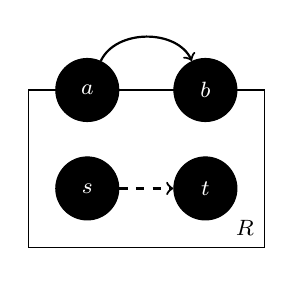
\begin{tikzpicture}[every node/.style={draw,circle, fill=black, text=white, minimum size=0.8cm}, node distance=1.5cm]
            \footnotesize 
            \draw (-0.75, 0) rectangle (2.25,-2);
            \node (a') at (0,0) { $a$};
            \node(b') [right of=a'] {$b$};
            \node(a) at (0,-1.25) {$s$};
            \node(b) [right of=a] {$t$};
            \node[draw=none,fill=none, text=black] (R) at (2, -1.75) { $R$};
            
            \draw[out=65, in=115, thick, ->] (a') to (b');
            \draw[dashed, thick, ->] (a) to (b);
            \end{tikzpicture}
        \end{center}
        \caption{$t$ ist bereits in $R$ von $s$ aus erreichbar}
    \end{subfigure}    
    \begin{subfigure}[t]{.3\linewidth}
        \begin{center}
            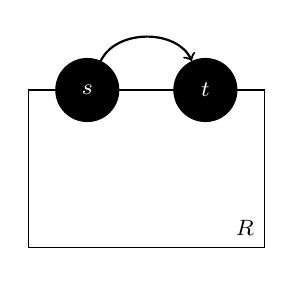
\begin{tikzpicture}[every node/.style={draw,circle, fill=black, text=white, minimum size=0.8cm}, node distance=1.5cm]
            \footnotesize 
            \draw (-0.75, 0) rectangle (2.25,-2);
            \node (a') at (0,0) { $s$};
            \node(b') [right of=a'] {$t$};
            %\node(a) at (0,-1.5) {$s$};
            %\node(b) [right of=a] {$t$};
            \node[draw=none,fill=none, text=black] (R) at (2, -1.75) { $R$};
            
            \draw[out=65, in=115, thick, ->] (a') to (b');
            %\draw[dashed, thick, ->] (a) to (b);
            \end{tikzpicture}
        \end{center}
        \caption{$s=a$ und $t=b$}
    \end{subfigure}    
    \begin{subfigure}[t]{.3\linewidth}
        \begin{center}
            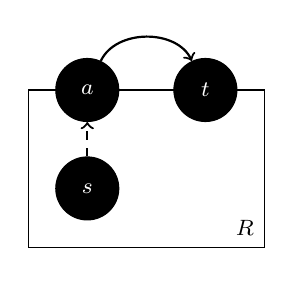
\begin{tikzpicture}[every node/.style={draw,circle, fill=black, text=white, minimum size=0.8cm}, node distance=1.5cm]
            \footnotesize 
            \draw (-0.75, 0) rectangle (2.25,-2);
            \node (a') at (0,0) { $a$};
            \node(b') [right of=a'] {$t$};
            \node(a) at (0,-1.25) {$s$};
            %\node(b) [right of=a] {$t$};
            \node[draw=none,fill=none, text=black] (R) at (2, -1.75) { $R$};
            
            \draw[out=65, in=115, thick, ->] (a') to (b');
            \draw[dashed, thick, ->] (a) to (a');
            \end{tikzpicture}
        \end{center}
        \caption{Es gibt in $R$ einen Pfad von $s$ zu $a$ und $t=b$}
    \end{subfigure}
    \begin{subfigure}[t]{.3\linewidth}
        \begin{center}
            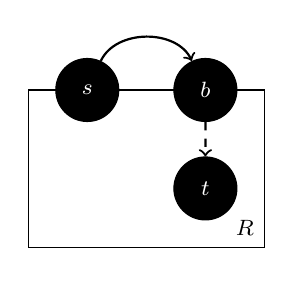
\begin{tikzpicture}[every node/.style={draw,circle, fill=black, text=white, minimum size=0.8cm}, node distance=1.5cm]
            \footnotesize 
            \draw (-0.75, 0) rectangle (2.25,-2);
            \node (a') at (0,0) { $s$};
            \node(b') [right of=a'] {$b$};
            %\node(a) at (0,-1.5) {$s$};
            \node(b) at (1.5,-1.25) {$t$};
            \node[draw=none,fill=none, text=black] (R) at (2, -1.75) { $R$};
            
            \draw[out=65, in=115, thick, ->] (a') to (b');
            \draw[dashed, thick, ->] (b') to (b);
            \end{tikzpicture}
        \end{center}
        \caption{Es gibt in $R$ einen Pfad von $b$ zu $t$ und $s=a$}
    \end{subfigure}
    \begin{subfigure}[t]{.3\linewidth}
        \begin{center}
            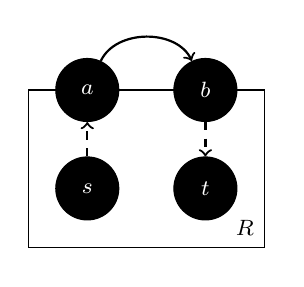
\begin{tikzpicture}[every node/.style={draw,circle, fill=black, text=white, minimum size=0.8cm}, node distance=1.5cm]
            \footnotesize 
            \draw (-0.75, 0) rectangle (2.25,-2);
            \node (a') at (0,0) { $a$};
            \node(b') [right of=a'] {$b$};
            \node(a) at (0,-1.25) {$s$};
            \node(b) [right of=a] {$t$};
            \node[draw=none,fill=none, text=black] (R) at (2, -1.75) { $R$};
            
            \draw[out=65, in=115, thick, ->] (a') to (b');
            \draw[dashed, thick, ->] (b') to (b);
            \draw[dashed, thick, ->] (a) to (a');
            \end{tikzpicture}
        \end{center}
        \caption{Es gibt in $R$ einen Pfad von $s$ zu $a$ und einen Pfad von $b$ zu $t$.}
    \end{subfigure}
    \caption{Erreichbarkeit im Graphen $(a,b)::R$}
    \label{fig:reach}
\end{figure}
\begin{enumerate}[label=(\alph*)]
    \item $t$ ist bereits in $R$ von $s$ aus erreichbar
    \item $s=a$ und $t=b$
    \item Es gibt in $R$ einen Pfad von $s$ zu $a$ und $t=b$
    \item Es gibt in $R$ einen Pfad von $b$ zu $t$ und $s=a$
    \item Es gibt in $R$ einen Pfad von $s$ zu $a$ und einen Pfad von $b$ zu $t$.
\end{enumerate}

Dies können wir im Form des folgenden Lemmas in \Cref{lst:t_path_trans_R_and} formalisieren.

\begin{code}[t_path_trans_R_and]{Utils.v}{}{1265}
Lemma t_path_trans_R_and {A} {eqdec: EqDec A eq} : 
    forall R (s t a b : A) P',
      t_path ((a, b)::R) P' s t ->
        {P & t_path R P s t} + 
        {(a, b) = (s, t)} +
        {P & prod (t_path R P s a) (t = b)} +
        {P & prod (t_path R P b t) (s = a)} +
        {P1 & {P2 & prod (t_path R P1 s a) (t_path R P2 b t)}}.
\end{code}

Mithilfe von \coqrefnl{t_path_trans_R_and} können wir nun die Entscheidbarkeit von \coqrefnl{t_path} beweisen.

\begin{code}[t_path_dec]{Utils.v}{}{1301}
Lemma t_path_dec {A} {eqdec : EqDec A eq} : forall R (s t : A), 
    {P & t_path R P s t} + {forall P, (t_path R P s t -> False)}.
\end{code}
Das Lemma in \Cref{lst:t_path_dec} kann nun durch Induktion über $R$ bewiesen werden. Der Fall für die leere Relation gilt trivialerweise, $t$ ist nicht von $s$ aus erreichbar. Im Induktionsschritt $R \leadsto (a,b)::R$ kann nun jeder Fall aus \Cref{fig:reach} getestet werden und, falls keiner dieser Fälle zutrifft, kann mittels \coqref{t_path_trans_R_and} gezeigt werden, dass \icoq{t} von \icoq{s} aus nicht erreichbar ist.

Durch die Entscheidbarkeit der Pfadkonstruktion und den Überführungen \coqref{t_path_ex} und \coqreff{lst:t_path_ex}{t_path_trh} lässt sich direkt die Entscheidbarkeit des transitiven Abschlusses zeigen.

\begin{code}[trans_hull_dec]{Utils.v}{}{1331}
Lemma trans_hull_dec {A} {eqdec: EqDec A eq}: forall R (s t :A), 
    trans_hull R s t + (trans_hull R s t -> False).
\end{code}

Es bleibt nun noch zu zeigen, dass aus der Entscheidbarkeit des transitiven Abschlusses und der Entscheidbarkeit der symmetrischen Abschlusses die Entscheidbarkeit des transitiv-symmetrischen Abschlusses folgt. Dafür zeigen wir zunächst die Äquivalenz zwischen \coqref{trans_hull} angewendet auf \coqref{sym_hull_list} und \coqref{ts_cl_list}.

\begin{multicode}[ts_cl_list_trans_sym]{Utils.v}{}{\texttt{ts\_cl\_list\_trans\_sym} und \texttt{trans\_sym\_ts\_cl\_list}}
\begin{mcode}{1056}
Lemma ts_cl_list_trans_sym {A} {eqdec: EqDec A eq} : 
    forall R (s t : A), ts_cl_list R s t ->
      trans_hull (sym_hull_list R) s t.
\end{mcode}
\begin{mcode}{1075}
Lemma trans_sym_ts_cl_list {A} {eqdec: EqDec A eq} : 
    forall R (s t : A), trans_hull (sym_hull_list R) s t ->
      ts_cl_list R s t.
\end{mcode}
\end{multicode}

Über die Überführung aus \Cref{lst:ts_cl_list_trans_sym} sowie die Entscheidbarkeit von \coqrefnl{t_path} lässt sich direkt die Entscheidbarkeit des transitiv-symmetrischen Abschlusses zeigen.

\begin{code}[ts_cl_list_dec]{Utils.v}{}{1339}
Lemma ts_cl_list_dec {A} {eqdec: EqDec A eq}: forall R (s t: A), 
    ts_cl_list R s t + (ts_cl_list R s t -> False).
\end{code}

Zuletzt zeigen wir noch, dass der transitiv-symmetrischen Abschluss die Eigenschaft der \emph{inneren} Reflexivität erfüllt. Siehe hierzu auch die Bemerkung zu \Cref{def:rt}.

\begin{multicode}[almost_refl]{Utils.v}{}{\texttt{almost\_refl\_l} und \texttt{almost\_refl\_r}}
    \begin{mcode}{2075}
Lemma almost_refl_l {A} R : forall (a b :A), ts_cl_list R a b -> 
    ts_cl_list R a a.
    \end{mcode}
    \begin{mcode}{2081}
Lemma almost_refl_r {A} R : forall (a b :A), ts_cl_list R a b -> 
    ts_cl_list R b b.
    \end{mcode}
\end{multicode}
Der Beweis der beiden Aussagen aus \Cref{lst:almost_refl} folgt direkt durch die folgenden Implikationen:
\[(a,b)\in R \overset{\text{Sym.}}{\implies} (a,b), (b,a)\in R^{ts} \overset{\text{Trans.}}{\implies} (a,a), (b,b) \in R^{ts}\]

\subsection{Ableitung und Teilableitung}
Um nun den Teilformelkalkül definieren zu können, implementieren wir zunächst in \Cref{lst:make_tgt_path} eine Funktion, die uns Pfade in der Form  $\pi\cdot\tgt^{i-1}$ generiert, wie sie im applikativen Fall in \Cref{def:SfC} verwendet werden.
\begin{code}[make_tgt_path]{Paths.v}{}{261}
Definition make_tgt_path (pi: path) (n : nat) :=
    pi ++ (repeat Tgt n) ++ [Src].
\end{code}

Nun kann die Ableitung des Teilformelkalküls definiert werden. Auch diese ähnelt stark \coqref{nfty_long} und \coqref{nfty}.

\begin{code}[SfC]{SfC.v}{Siehe \Cref{def:SfC}}{20}
Inductive SfC (Delta : list path) (R: path -> path -> Type) : 
    nfterm -> path -> Type :=
  | SfC_I s pi : SfC ((pi ++ [Src]) :: Delta) R s (pi ++ [Tgt]) ->
      SfC Delta R (\__ s) pi
  | SfC_E ms pi pi' x : nth_error Delta x = Some pi -> 
      R (pi ++ repeat Tgt (length ms)) pi'  ->
        (forall n (p: n < length ms), 
            SfC Delta R (nth_ok ms n p) (make_tgt_path pi n) ) ->
          SfC Delta R (!! x @@ ms) pi'.
\end{code}

Da wir für einige Beweise explizit Teilableitungen von \coqrefnl{SfC} betrachten müssen, führen wir in \Cref{lst:SfC_subj} eine Relation ein, die Teilableitungen beschreibt.
\begin{code}[SfC_subj]{SfC.v}{}{304}
Inductive SfC_subj R : forall Delta Delta' m m' pi pi', 
    SfC Delta R m pi -> SfC Delta' R m' pi' -> Type :=
  | SfC_subj_refl : forall Delta m pi (proof: SfC Delta R m pi), 
      SfC_subj _ _ _ _ _ _ _ proof proof
  | SfC_subj_trans : forall Delta Delta' Delta'' m m' m'' pi pi' pi'' 
      (proof1 : SfC Delta R m pi) 
      (proof2: SfC Delta' R m' pi') 
      (proof3: SfC Delta'' R m'' pi''),
        SfC_subj _ _ _ _ _ _ _ proof1 proof2 ->
          SfC_subj _ _ _ _ _ _ _ proof2 proof3 ->
            SfC_subj _ _ _ _ _ _ _ proof1 proof3
  | SfC_subj_I : forall Delta m pi (proof: SfC ((pi ++ [Src]) :: Delta) 
      R m (pi ++ [Tgt])),
        SfC_subj _ _ _ _ _ _ _ proof (SfC_I _ _ _ _ proof)
  | SfC_subj_E : forall Delta pi pi' ms x
      (deltaok: nth_error Delta x = Some pi)
      (Rproof: R (pi ++ repeat Tgt (length ms)) pi')
      (proofs: (forall n (p: n < length ms), 
        SfC Delta R (nth_ok ms n p) (make_tgt_path pi n) ))
      n (ltproof: (n < length ms)),
    SfC_subj _ _ _ _ _ _ _ (proofs n ltproof) 
       (SfC_E _ _ _ _ _ _ deltaok Rproof proofs).    
\end{code}
Während \icoq{SfC_subj_refl} und \icoq{SfC_subj_trans} den reflexiven bzw. transitiven Abschluss einer Teilableitung beschreiben, beschreiben \icoq{SfC_subj_I} und \icoq{SfC_subj_E} genau einen Schritt einer Ableitung. Die übergebenen Argumente der Konstruktoren der Teilableitung werden lediglich an die Konstruktoren des Teilformelkalküls (\Cref{lst:SfC}) weitergeleitet. 

Des Weiteren benötigen wir für den Beweis von \Cref{lem:evenodd}, eine Möglichkeit Aussagen über jeden  einzelnen Schritt einer Ableitung zu formulieren. Hierfür formulieren wir in \Cref{lst:each_judg_SfC} eine Funktion, die eine Aussage \icoq{P} über einzelne Ableitungsschritte und einer Pfadableitung \icoq{proof} entgegennimmt und eine Konjunktion über alle Schritte der Ableitung generiert.
\begin{code}[each_judg_SfC]{SfC.v}{}{357}
Fixpoint each_judg_SfC {Delta R m pi} 
  (P : forall Delta' R' m' pi', SfC Delta' R' m' pi' -> Prop) 
  (proof : SfC Delta R m pi) : Prop :=
    P Delta R m pi proof /\
      match proof with
      | SfC_I _ _ s' pi' proof' => each_judg_SfC (P) proof'
      | SfC_E _ _ ms pi pi' x DeltaProof Rproof proof' =>
          forall (n : nat) (p : n < length ms),
            each_judg_SfC (P) (proof' n p)
      end.
\end{code}

Da \coqrefnl{each_judg_SfC} Aussagen über alle Teilableitungen einer Ableitung trifft, lässt sich ein Zusammenhang zu Konstruktion \coqref{SfC_subj} herstellen.
\begin{multicode}[each_judg_subj_SfC]{SfC.v}{}{\texttt{each\_judg\_subj\_SfC} und \texttt{each\_judg\_subj\_SfC\_P}}
    \begin{mcode}{366}
Lemma each_judg_subj_SfC : forall Delta R t pi (m : SfC Delta R t pi) P,
    each_judg_SfC P m ->
      forall Delta' t' pi' (n : SfC Delta' R t' pi'), 
        SfC_subj _ _ _ _ _ _ _ n m ->
          (each_judg_SfC P n).
\end{mcode}
\pagebreak   
\begin{mcode}{381}
Lemma each_judg_subj_SfC_P : forall Delta R t pi (m : SfC Delta R t pi) P,
    each_judg_SfC P m ->
      forall Delta' t' pi' (n : SfC Delta' R t' pi'), 
        SfC_subj _ _ _ _ _ _ _ n m ->
          P _ _ _ _ n.
\end{mcode}
\end{multicode}
\begin{remark}
    Die beiden Lemmata in \Cref{lst:each_judg_subj_SfC} zeigen sehr ähnliche Aussagen, die an unterschiedlichen Stellen benötigt werden. \icoq{each_judg_SfC} zeigt die allgemeinere Aussage, dass, wenn für zwei Ableitungen \icoq{m} und \icoq{n} gilt, dass \icoq{n} eine Teilableitung nach \coqref{SfC_subj} von \icoq{m} ist und eine Aussage \icoq{P} für \icoq{m} und alle Teilableitngen nach \coqref{each_judg_SfC} gilt, dann gilt sie auch für alle Teilableitungen von \icoq{n}.
    
    Das zweite Lemma ist ein Spezialfall des ersten und sagt lediglich aus, dass in diesem Fall die Aussage für \icoq{n} gilt.
\end{remark}
Das erste Lemma in \Cref{lst:each_judg_subj_SfC} kann durch Induktion über \coqref{SfC_subj} bewiesen werden. Das zweite Lemma wird mit dem ersten bewiesen.

Mittels des in \Cref{lst:each_judg_impl} aufgestellten Lemmas kann eine Implikation von Aussagen $P$ und $Q$ auf Einzelschritten einer Ableitung auf die Implikation der Aussagen auf dem gesamten Ableitungsbaum geliftet werden. Dies wird für den Zusammenhang zwischen \Cref{lem:evenodd} und \Cref{cor:norefl} benötigt.
\begin{code}[each_judg_impl]{SfC.v}{}{459}
Lemma each_judg_impl : forall 
    (P : forall Delta R m pi, SfC Delta R m pi -> Prop)
    (Q : forall Delta R m pi, SfC Delta R m pi -> Prop), 
  (forall Delta R m pi (proof : SfC Delta R m pi), 
      P _ _ _ _ proof ->  Q _ _ _ _ proof) -> 
    forall Delta R m pi (proof : SfC Delta R m pi), 
      each_judg_SfC P proof -> each_judg_SfC Q proof.
\end{code}

Für den Beweis von \Cref{lem:fz} wird ein Generierungslemma des Teilformelkalküls benötigt. Intuitiv ist klar, dass ein \coqref{nfterm} der Form \icoq{\__ m} mit dem Konstruktor \coqreff{lst:SfC}{SfC_I} und ein \coqrefnl{nfterm} der Form \icoq{!! x @@ ms} mit dem Konstruktor \coqreffnl{lst:SfC}{SfC_E} bewiesen wird. Mit den Lemmata aus \Cref{lst:SfC_gen} kann diese Intuition formalisiert werden.
\begin{multicode}[SfC_gen]{SfC.v}{}{\texttt{SfC\_gen\_app} und \texttt{SfC\_gen\_lam}}
\begin{mcode}{90}
Lemma SfC_gen_app : forall R x ms pi' Delta 
    (proof : SfC Delta R (!! x @@ ms) pi'),    
  SfC_E Delta R ms
    (get_subproof_app_pi proof) pi' x
      (get_subproof_app_deltaok proof)
        (get_subproof_app_Rok proof)
          (get_subproof_app proof) = proof.
\end{mcode}
\begin{mcode}{214}
Lemma SfC_gen_lam R m pi Delta (proof : SfC Delta R (\__ m) pi) :
    SfC_I Delta R m pi (get_subproof_lam proof) = proof .
\end{mcode}
\end{multicode}
\begin{remark}
    \begin{itemize}
        \item Die mit \icoq{get_subproof_} gepräfixten Funktionen extrahieren aus einem gegebenen Beweis genau die entsprechenden Teilbeweise.
        \item Für den Beweis dieser beiden Lemmata war es notwendig, einen großen Teil des Beweises explizit als \tlambda-Term anzugeben (Siehe \Cref{sec:IPC}), da die Taktiksprache von \coq{} keinen entsprechenden Beweis formulieren konnte. Dadurch ist der implementierte Beweis sehr umständlich und schwer nachzuvollziehen. Im Kern wird lediglich eine Fallunterscheidung über \icoq{proof} durchgeführt und ein Fall wird ad absurdum geführt.
    \end{itemize}
\end{remark}

\subsection{Eigenschaften der Pfadrelationen}

Wir betrachten nun die Eigenschaften, die Pfadrelationen haben. Insbesondere werden wir dabei \Cref{cor:norefl} formalisieren und beweisen. Zunächst formulieren wir in \Cref{lst:sfc_monotone} auf Basis von \coqref{Rsub} das Monotonielemma \ref{lem:mono}, das später benötigt wird, um die Korrektheit der Implementierung von \Cref{alg:rm} zu beweisen. Analog zu \coqrefnl{Rsub} formulieren wir auch ein Lemma für die Behandlung als Liste.

\begin{multicode}[sfc_monotone]{SfC.v}{Siehe \Cref{lem:mono}}{\texttt{sfc\_monotone\_aux}, \texttt{sfc\_monotone} und \texttt{sfc\_monotone\_aux\_list}}
    \begin{mcode}{321}
Lemma sfc_monotone_aux : forall m R R' pi Delta, Rsub R R' ->
    SfC Delta R m pi -> SfC Delta R' m pi.
    \end{mcode}
    \begin{mcode}{334}
Lemma sfc_monotone : forall m R R', Rsub R R' -> 
    SfC [] R m [] -> SfC [] R' m [].
    \end{mcode}
    \begin{mcode}{342}
Lemma sfc_monotone_aux_list : forall m R R' pi Delta, Rsub_list R R' ->
    SfC Delta (ts_cl_list R) m pi ->
      SfC Delta (ts_cl_list R') m pi.
    \end{mcode}
\end{multicode}
\begin{remark}
    \begin{itemize}
        \item \icoq{sfc_monotone_aux} ist die verallgemeinerte Variante von \icoq{sfc_monotone} für beliebige Pfadkontexte $\Delta$. 
        \item  Für die Listendarstellung ist nur das verallgemeinerte Lemma implementiert. Eine Variante für den leeren Pfadkontext wird nicht benötigt.
    \end{itemize}
\end{remark}    
\coqreff{lst:sfc_monotone}{sfc_monotone_aux} lässt sich direkt über Induktion von \icoq{SfC Delta R m pi} beweisen. \coqrefnl{sfc_monotone} sowie \icoq{sfc_monotone_aux_list} können direkt über das erste Lemma bewiesen werden.

Im Folgenden werden wir \Cref{cor:norefl} formulieren und für den Beweis die notwendigen Lemmata aufstellen. Zunächst stellen wir die Bedingung, die in \Cref{lem:evenodd} verwendet wird, für einen einzelnen gegebenen Ableitungschritt auf. Die hierfür notwendigen Teilbedingungen, dass einerseits die Anzahl an \src{} gerade in $\pi$ und dass die Anzahl an \src{} ungerade in einem Pfad im Kontext ist, werden in \Cref{lst:even_ones} formalisiert.

\begin{multicode}[even_ones]{Paths.v}{}{\texttt{even\_ones} und \texttt{odd\_repo}}
    \begin{mcode}{264}
Definition even_ones pi := Nat.Even (count_occ dir_eqdec pi Src).
    \end{mcode}
    \begin{mcode}{274}
Definition odd_repo (Delta : list path) := 
    Forall (fun pi => Nat.Odd (count_occ dir_eqdec pi Src)) Delta.
    \end{mcode}
\end{multicode}

Nun kann eine Bedingung für Ableitungsschritte von \coqref{SfC} angegeben werden, welche die einzelnen Bedingungen aus \Cref{lst:even_ones} vereint.
\begin{code}[evenodd_cond]{SfC.v}{}{383}
Definition evenodd_cond {Delta R m pi} (proof : SfC Delta R m pi) :=
    (even_ones pi) /\ (odd_repo (Delta)).
\end{code}
Um nun zu fordern, dass jeder Ableitungsschritt einer Ableitung diese Bedingung erfüllt, kann die Konstruktion \coqref{each_judg_SfC} genutzt werden, und so \Cref{lem:evenodd} in \Cref{lst:evenodd} formalisiert werden.
\begin{code}[evenodd]{SfC.v}{Siehe \Cref{lem:evenodd}}{423}
Lemma evenodd {R m} (proof : SfC [] R m []) : 
    each_judg_SfC (@evenodd_cond) proof.
\end{code}
Der Beweis hierfür folgt analog zu dem Beweis in \Cref{lem:evenodd} über die in \Cref{lst:evenodd_aux} formalisierte allgemeinere Aussage.
\begin{code}[evenodd_aux]{SfC.v}{}{400}
Lemma evenodd_aux {Delta R m pi} (proof : SfC Delta R m pi) : 
    evenodd_cond proof -> each_judg_SfC (@evenodd_cond) proof.
\end{code}
Dies kann durch Induktion über \icoq{proof} und Auflösen der \coqrefnl{each_judg_SfC} Konstruktion sowie einiger Regeln über gerade und ungerade Pfade bewiesen werden.

Die Bedingung aus \Cref{cor:norefl}, dass kein Ableitungsschritt die Bedingung $(\pi,\pi)\in R$ hat, wird ebenfalls zunächst auf einem einzelnen Ableitungsschritt formuliert, um dann mit \coqrefnl{each_judg_SfC} auf die ganze Ableitung geliftet zu werden. Wir betrachten hier die Konstruktoren von \coqref{SfC} einzeln. Der Konstruktor für die Applikation stellt keine Anforderungen an \icoq{R}, somit kann in diesem Fall immer \icoq{True} zurückgegeben werden. Für den applikativen Fall reicht es zu fordern, dass $\pi' \neq \pi\cdot\tgt^n$ gilt.
\begin{code}[r_not_refl_cond]{SfC.v}{}{432}
Definition r_not_refl_cond {Delta R m pi} (proof : SfC Delta R m pi)  :=
  match proof with
  | SfC_I _ _ _ _ _ => True
  | SfC_E _ _ ms pi pi' _ _ _ _ => 
      ~ (pi ++ repeat Tgt (length ms) = pi')
  end.
\end{code}

Wir können nun zeigen, dass aus \coqref{evenodd_cond} die Bedingung \coqref{r_not_refl_cond} folgt. 
\begin{code}[evenodd_2_r_not_refl]{SfC.v}{}{438} 
Lemma evenodd_2_r_not_refl {Delta R m pi} (proof : SfC Delta R m pi) : 
    evenodd_cond proof -> r_not_refl_cond proof.
\end{code}

Mittels \coqref{each_judg_impl} kann \coqref{evenodd_2_r_not_refl} auf die gesamte Ableitung geliftet werden. Da \coqref{evenodd} gilt, gilt auch das folgende Lemma.
\begin{code}[r_not_refl]{SfC.v}{Siehe \Cref{cor:norefl}}{473}
Lemma r_not_refl {R m} (proof : SfC [] R m []) : 
    each_judg_SfC (@r_not_refl_cond) proof.
\end{code}

\subsection{Verifikation des Algorithmus $R_M$-aux}

In diesem Abschnitt werden wir die Implementierung des \Cref{alg:rm} betrachten sowie seine Korrektheit und Minimalität beweisen. Hierfür betrachten wir zunächst die Implementierung des Algorithmus in \Cref{lst:R_m_aux}.
\begin{code}[R_m_aux]{SfC.v}{Siehe \Cref{alg:rm}}{491}
Fixpoint R_m_aux (Delta: list path) (pi': path) (m : nfterm) 
  {struct m} : option (list (path * path)) :=
    match m with
    | \__ s => R_m_aux ((pi' ++ [Src]) :: Delta) (pi' ++ [Tgt]) s
    | !! x @@ ms => 
        match nth_error Delta x with
        | None => None
        | Some pi => 
           option_concat (combine_with 
            (fun x n => R_m_aux Delta (make_tgt_path pi n) x)
            ms (range (length ms)) ++
             [Some [((pi ++ repeat Tgt (length ms), pi'))]])
        end
     end.
\end{code}
\begin{remark}
    \begin{itemize}
        \item \icoq{option_concat}, \icoq{combine_with} sowie \icoq{range} sind in \texttt{Utils.v} definierte Hilfsfunktionen. 
        \begin{itemize}
            \item \icoq{option_concat : list (option (list A)) -> option (list A)} gibt \icoq{None} zurück, wenn mindestens ein Element der Eingabe \icoq{None} ist. Ansonsten werden alle Listen konkateniert und im \icoq{option} Datentyp gekapselt.
            \item \icoq{combine_with (f: (A -> B -> C)) : list A -> list B -> list C} arbeitet wie \icoq{combine}, nur, dass nicht eine Liste von Tupeln \icoq{(A * B)} generiert wird, sondern jedes Element der Rückgabeliste von der Funktion \icoq{f} generiert wird.
            \item \icoq{range n : list nat} ist direkt über \icoq{seq 0 n} definiert.
        \end{itemize}
        \item In \texttt{SfC.v} wird anstelle der Funktion \icoq{combine_with} aus \texttt{Utils.v} ein Fixpunkt \emph{inline} mit dem Namen \icoq{combine_with} definiert, der sich genau so verhält. Dies muss auf diese Weise gelöst werden, damit \coq{} erkennt, dass im Rekursionsschritt \icoq{m} strukturell kleiner wird. Das Lemma \icoq{combine_with_inline} zeigt die Gleichheit der beiden Formulierungen.
    \end{itemize}
\end{remark}

Des Weiteren betrachten wir hier noch einige Definitionen, die den Aufruf an \coqrefnl{R_m_aux} kapseln. 
Zum einen benötigen wir einen initalen Aufruf ohne Kontext, zum anderen benötigen wir den transitiv-symmetrische Abschluss mittels \coqref{ts_cl_list}. Bei letzterem ist zu beachten, dass \coqrefnl{R_m_aux} \icoq{None} zurückgibt, falls der Algorithmus fehlschlägt. In diesem Fall interpretieren wir den Abschluss als Funktion, die immer \icoq{False} zurückgibt.
\begin{multicode}[R_m]{SfC.v}{}{\texttt{R\_m} und \texttt{R\_m\_ts}}
    \begin{mcode}{510}
Definition R_m m := R_m_aux [] [] m.
\end{mcode}
\begin{mcode}{514}
Definition R_m_ts m := match R_m m with
  | None => fun pi pi' => False
  | Some Rmm => ts_cl_list (Rmm)
end.
\end{mcode}
\end{multicode}

Wir beweisen nun die Korrektheit des Algorithmus aus, also dass, falls der Algorithmus erfolgreich terminiert, die über \coqref{R_m_aux} generierten Relationen, zu einer korrekten Typableitung führt. 

\begin{code}[R_m_ts_correct]{SfC.v}{Siehe \Cref{lem:rmauxcorrect}}{567}
Lemma R_m_ts_correct : forall m Rm Delta pi, 
    R_m_aux Delta pi m = Some Rm  -> 
      SfC Delta (ts_cl_list Rm) m pi.
\end{code}
Das in \Cref{lst:R_m_ts_correct} formulierte Lemma kann durch Induktion über \icoq{m} bewiesen werden. Der Abstraktionsfall ist trivial, da hier die Relation nicht genutzt wird. Im Applikationsfall kann dadurch, dass \icoq{R_m_aux Delta pi m = Some Rm} gefordert wird, die durch \icoq{option_concat} und \icoq{combine_with} konstruierte Liste auseinander genommen werden und immer gezeigt werden, dass niemals \icoq{None} das Ergebnis eines rekursiven Aufrufs war. Die Applikation kann dann durch den Konstruktor von \coqref{SfC} auseinander genommen werden und es kann gezeigt werden, dass das geforderte Tupel  \icoq{(pi ++ repeat Tgt (length ms), pi')} im entsprechenden Schritt hinzugefügt wird. 

Da der Induktionschritt über \coqref{nfterm} durchgeführt wird, wird zwar \icoq{m} destruiert, die Pfadrelation wird jedoch nicht für den induktiven Abstieg angepasst. Hier wird \coqref{sfc_monotone} genutzt, um zu zeigen, dass eine Ableitung auch mit einer größeren Relation durchführbar ist.

Es bleibt zu zeigen, dass die von \coqrefnl{R_m_aux} generierte Relation auch die kleinste Relation ist.
\begin{code}[R_m_ts_minimal]{SfC.v}{Siehe \Cref{def:rm,lem:rmauxcorrect}}{805}
Lemma R_m_ts_minimal : forall m Rm Delta pi,  
    SfC Delta Rm m pi -> forall Rm', R_m_aux Delta pi m = Some Rm' -> 
      Rsub (fun p p' => In (p, p') Rm') Rm.
\end{code}
Dies kann direkt durch Induktion über \coqrefnl{SfC} bewiesen werden. Der Abstraktionsfall ist hier ebenfalls trivial. Im Applikationsfall kann analog zu \coqrefnl{R_m_ts_correct} die Liste der Subaufrufe auseinandergenommen werden, da gefordert ist, dass \coqrefnl{R_m_aux} erfolgreich terminiert.

Sowohl \coqrefnl{R_m_ts_correct} als auch \coqrefnl{R_m_ts_minimal} fordern, dass \coqref{R_m_aux} erfolgreich terminiert. Wir werden hier abschließend noch die hinreichende Bedingung aus \Cref{lem:rmclosed} formalisieren, nach der \coqrefnl{R_m_aux} erfolgreich terminiert, wenn der entsprechende \coqrefnl{nfterm} \coqref{closed} ist. Dies kann über die allgemeinere Aussage bewiesen werden, dass \coqrefnl{R_m_aux} nicht fehlschlägt, wenn der übergebene Kontext allen freien Variablen einen Pfad zuweist. Hierfür wird \coqref{all_var_in_repo} genutzt.

\begin{code}[exists_R_m]{SfC}{Siehe \Cref{lem:rmclosed}}{654}
Lemma exists_R_m m : forall Delta, all_var_in_repo m Delta -> 
    forall pi, { R' & R_m_aux Delta pi m = Some R'}.
\end{code}
Der Beweis für das Lemma in \Cref{lst:exists_R_m} wird durch Induktion über \icoq{m} geführt. Der Abstraktionsfall ist erneut trivial. Für Applikationsfall kann die Hypothese darauf heruntergebrochen werden, dass sowohl die initiale Variable im Kontext ist sowie, dass die Hypothese für jeden einzelnen Term der Applikation gilt. Über die Induktionshypothese kann somit die Gesamtaussage für jeden einzelnen Term der Applikation gezeigt werden. Es kann nun weiter gezeigt werden, dass sich diese Einzelresultate kombinieren lassen, sodass das Lemma gezeigt ist.

Grundsätzlich können die hier vorgestellten Lemmata zu der in \Cref{lst:closed_Rm} formulierten Aussage erweitert werden.
\begin{code}[closed_Rm]{SfC.v}{}{724}
Lemma closed_Rm : forall m, closed m -> SfC [] (R_m_ts m) m [].  
\end{code}
Es gilt sogar die umgedrehte Richtung, und eine vergleichbare Aussage für \coqref{nfty_long}. Die Beweise für beide Aussagen werden jeweils über ein Zwischenlemma geführt, das den allgemeineren Fall beweist und ähneln sich sehr stark. Dies liegt an der strukturellen Ähnlichkeit der beiden Ableitungen.
\begin{multicode}[SfC_closed]{SfC.v}{}{\texttt{SfC\_closed} und \texttt{Long\_closed}}
   \begin{mcode}{763}
Lemma SfC_closed : forall R m, SfC [] R m [] -> closed m.
\end{mcode}
\begin{mcode}{799}
Lemma Long_closed : forall m rho, nfty_long [] m rho -> closed m.
\end{mcode}
\end{multicode}

\subsection{Implementierung der typabhängigen Relation}

Im Folgenden wird die typabhängige Relation $R_\tau$ formalisiert. Im Gegensatz zu $R_M$ bedarf es hier keines Algorithmus. Wir werden an dieser Stelle die notwendige Bedingung an ein Tupelpaar formulieren, um anschließend die Liste aller gültigen Pfade zu einem Typen über diese Bedingung zu filtern. Da die \icoq{filter}-Funktion der \coq{}-Standardbibliothek die Filterbedingung als Funktion mit Zieltyp \icoq{bool} erwartet, ist die Bedingung als solche formuliert. 
\begin{code}[R_tau_cond]{SfC.v}{Siehe \Cref{def:rt}}{850}
Definition R_tau_cond (tau: type) (pipi' : path * path) : bool :=
  let pi := fst pipi' in
  let pi' := snd pipi' in
  (pi <>b pi') && 
    match P tau pi with
    | None => false
    | Some (sigma ~> tau) => false
    | Some (? a) => match P tau pi' with
        | None => false
        | Some a' => (? a) ==b a'
        end
    end.
\end{code}

Die Menge aller gültigen Pfade in einem Typen ist genau der Definitionsbereich der Funktion $P_\tau$, der hier der Rückgabe der Funktion \coqref{dom_P} entspricht.

\begin{code}[R_tau_list]{SfC.v}{Siehe \Cref{def:rt}}{864}
Definition R_tau_list tau :=
    filter (R_tau_cond tau)
      (list_prod (dom_P tau) (dom_P tau)).
\end{code}

Auch für \coqref{R_tau_list} benötigen wir den transitiv-symmetrischen Abschluss über \coqref{ts_cl_list}.

\begin{code}[R_tau_ts]{SfC.v}{Siehe \Cref{def:rt}}{875}
Definition R_tau_ts (tau: type) := ts_cl_list (R_tau_list tau).
\end{code}

\subsection{Zusammenhang von Langableitung und Teilformelkalkül}

Als letztes Lemma wird hier \Cref{lem:fz}, der Zusammenhang zwischen der Langableitung und des Teilformelkalküls, formalisiert. Ein wichtiger Mechanismus für den Beweis ist es, Pfadableitungen in Typableitungen zu überführen. Dafür definieren wir in \Cref{lst:Delta2Gamma} zunächst eine Funktion, die Pfadkontexte in Typkontexte zu einem gegebenen Typen überführt.

\begin{code}[Delta2Gamma]{SfC.v}{}{901}
Definition Delta2Gamma (tau: type) Delta : option (list type) :=
    all_some (map (P tau) Delta).    
\end{code}
\begin{remark}
    \icoq{all_some : list (option A) -> option (list A)} ist \icoq{None}, wenn in der übergebenen Liste mindestens ein \icoq{None} vorkommt, ansonsten werden die Elemente aus dem \icoq{option} Datentyp ausgepackt und zurückgegeben.
\end{remark}

Im Kern des Beweises für \textbf{1 $\implies$ 2} (\Cref{lem:fz}) zeigen wir, dass wir in $\vdash_R$ die Relation $R$ durch eine Relation $R'$ ersetzen können, wenn alle relevanten Tupel auch in $R'$ sind. Da die Applikationsregeln bestimmen, welche Tupel relevant sind, brauchen wir nur diese Teilschritte betrachten. Dies kann als Hilfslemma formuliert werden. 

\begin{code}[sfc_replace_R]{SfC.v}{}{1160}
Lemma sfc_replace_R {R m Delta' pi''}: 
    forall (base_sfc: SfC Delta' R m pi'') R',
        (forall Delta x pi, nth_error Delta x = Some pi -> 
          forall ms pi' (subj_sfc: SfC Delta R (!!x @@ ms) pi'), 
      SfC_subj _ _ _ _ _ _ _ subj_sfc base_sfc -> 
        R' (pi ++ repeat Tgt (length ms)) pi') -> 
          SfC Delta' R' m pi''.
\end{code}
Das Hilfslemma aus \Cref{lst:sfc_replace_R} kann durch Induktion über \icoq{base_sfc} sowie über die anschließende Verwendung der Hypothese \icoq{(forall Delta x pi, nth_error Delta x = Some pi -> forall ms pi' (subj_sfc: SfC Delta R (!!x @@ ms) pi')}, bewiesen werden. 

Es bleibt zu zeigen, dass, falls ein Term langtypbar ist, dieser genau diese Hypothese mit der Relation \coqref{R_tau_ts} erfüllt. Um zu zeigen, dass dies aus den einzelnen Teilschritten einer Langableitung folgt, müssen wir zunächst die einzelnen Teilschritte dieser explizit betrachten. Dafür nutzen wir die strukturelle Ähnlichkeit zwischen der Lang- und der Pfadableitung und erstellen aus Teilschritten der Pfadableitungen Teilschritte der Langableitung. Hierfür verwenden wir die eingangs definierte Funktion \coqref{Delta2Gamma}.

\begin{code}[sfc_to_long_subj]{SfC.v}{}{1032}
Lemma sfc_to_long_subj {rho} : 
    forall Delta R m pi (base_sfc : SfC Delta R m pi) Gamma,
      Delta2Gamma rho Delta = Some Gamma ->
        forall pr (base_long : nfty_long Gamma m (P_ok rho pi pr))
            Delta' m' pi' (subj_sfc : SfC Delta' R m' pi'),
          SfC_subj _ _ _ _ _ _ _ subj_sfc base_sfc ->
            { Gamma' & (Delta2Gamma rho Delta' = Some Gamma') *
              { pr' & nfty_long Gamma' m' (P_ok rho pi' pr')}}.
\end{code}

Der Beweis für das Lemma aus \Cref{lst:sfc_to_long_subj} folgt durch Induktion über die \coqrefnl{SfC_subj}-Relation (\Cref{lst:SfC_subj}). Während die Regeln für die Reflexivität, Transitivität und der Abstraktion einfach folgen, muss für die Applikation eine Induktion über die Liste der Typen durchgeführt werden, die in der Langableitung mit der Funktion \coqref{make_arrow_type} beschrieben werden.

Nun haben wir eine Möglichkeit, Schritte in Langableitungen und Pfadableitungen parallel zu betrachten. Dies erlaubt uns das in \Cref{lst:sfc_app_subj_types_atomic} aufgestellte Lemma zu beweisen, indem der Schritt in der Langableitung \icoq{base_long} analysiert wird, der zu dem Schritt \icoq{subj_sfc} in \icoq{base_sfc} korrespondiert.

\begin{code}[sfc_app_subj_types_atomic]{SfC.v}{}{1099}
Lemma sfc_app_subj_types_atomic {rho} : 
  forall R m someDelta somepi 
    (base_sfc : SfC someDelta R m somepi)
    someGamma somepr 
    (base_long : nfty_long someGamma m (P_ok rho somepi somepr))
    (someD2G: Delta2Gamma rho someDelta = Some someGamma)
    Delta x pi (Deltaok : nth_error Delta x = Some pi)
    ms pi' (subj_sfc : SfC Delta R (!! x @@ ms) pi'),
      SfC_subj _ _ _ _ _ _ _ subj_sfc base_sfc ->
        { a & P rho (pi ++ repeat Tgt (length ms)) = Some (? a) /\ 
            P rho (pi') = Some (? a) }.
\end{code}

Mit diesem Resultat lässt sich nun das folgende Lemma beweisen, dessen Resultat die gesuchte Hypothese für \coqref{sfc_replace_R} ist.

\begin{code}[sfc_app_subj_in_R_tau]{SfC.v}{}{1141}
Lemma sfc_app_subj_in_R_tau {rho m R} :
  forall (base_sfc : SfC [] R m []) (base_long : nfty_long [] m rho) 
    Delta x pi (Deltaok : nth_error Delta x = Some pi) ms pi'
      (subj_sfc : SfC Delta R (!! x @@ ms) pi'),
   SfC_subj _ _ _ _ _ _ _ subj_sfc base_sfc ->
        R_tau_ts rho (pi ++ repeat Tgt (length ms)) pi'.
\end{code}

Schließlich kann der erste Teil von \Cref{lem:fz} verifiziert werden.

\begin{code}[long_to_sfc_tau]{SfC.v}{Siehe \Cref{lem:fz} \textbf{1 $\implies$ 2}}{1188}
Lemma long_to_sfc_tau {rho m} : nfty_long [] m rho ->
    SfC [] (R_tau_ts rho) m [].
\end{code}
Über \coqreff{lst:SfC_closed}{Long_closed} wissen wir, dass \icoq{m} geschlossen ist. Weiter wissen wir über \coqref{closed_Rm}, dass der Term pfadableitbar mit $R_M$ ist. Über \coqref{sfc_app_subj_in_R_tau} und \coqref{sfc_replace_R} wissen wir, dass wir die Relation durch \icoq{R_tau_ts rho} ersetzen können. Somit gilt das Lemma in \Cref{lst:long_to_sfc_tau}.

Die Implementierung des Schrittes \textbf{2 $\implies$ 3}(\Cref{lem:fz}) kann analog zu dem entsprechenden Schritt in \Cref{lem:fz} bewiesen werden.

\begin{code}[sfc_tau_to_Rsub_m_tau]{SfC.v}{Siehe \Cref{lem:fz} \textbf{2 $\implies$ 3}}{1199}
Lemma sfc_tau_to_Rsub_m_tau {m tau} : 
    SfC [] (R_tau_ts tau) m [] -> Rsub (R_m_ts m) (R_tau_ts tau).
\end{code}

Wir wissen über \coqref{R_m_ts_minimal}, dass \icoq{R_m_ts m} Teilmenge jeder Relation ist, für die es eine Pfadableitung gibt. Somit insbesondere auch für \icoq{R_tau_ts rho}. Damit gilt auch \coqref{sfc_tau_to_Rsub_m_tau}.

Es bleibt, den Schritt \textbf{3 $\implies$ 1}(\Cref{lem:fz}) zu zeigen, also dass wir aus $R_M\subseteq R_\tau$ folgern können, dass $M$ mit $\tau$ im leeren Kontext langableitbar ist. Zunächst betrachten wir die wichtigsten Hilfslemmata, die im Beweis zu der Aussage genutzt werden.

Es kann gezeigt werden, dass, wenn ein Pfad ableitbar ist, dieser als Präfix in R verwendet wird.
\begin{code}[pi_in_R]{SfC.v}{}{1212}
Lemma pi_in_R : forall m Delta pi R, 
    SfC Delta R m pi -> {pi' & {app & R pi' (pi ++ app)}}.
\end{code}

Des Weiteren können wir folgen, dass für gültige Pfade, die auf \src{} enden, sowohl der Pfad ohne \src{} sowie der Pfad mit \tgt{} anstelle von \src{} gültig ist, und die entsprechenden Typen in Zusammenhang stehen.
\begin{code}[P_Src2]{Paths.v}{}{454}
Lemma P_Src2 : forall pi rho sigma, 
    P rho (pi ++ [Src]) = Some sigma -> 
      {tau & P rho pi = Some (sigma ~> tau) /\
        P rho (pi ++ [Tgt]) = Some tau}.
\end{code}

Wir können grundsätzlich die Aussage zeigen, dass, wenn ein Pfad in einem Typen gültig ist, auch jeder Präfix des Pfades in dem Typen gültig ist.
\begin{code}[P_prefix]{Paths.v}{}{144}
Lemma P_prefix {rho pi pi' rho'}: P rho (pi ++ pi') = Some rho' -> 
    {rho'' & P rho pi = Some rho''}.
\end{code}

Zudem gilt, dass es zu jedem gültigen Pfad, der auf \src{} endet, einen gültigen Pfad gibt, der auf \tgt{} endet, und umgekehrt.
\begin{code}[P_ok_replace_last]{Paths.v}{}{433}
Lemma P_ok_replace_last : forall pi rho dir1 dir2 pr1 sigma, 
    P_ok rho (pi ++ [dir1]) pr1 = sigma ->
      {pr2 & {rho' & P_ok rho (pi ++ [dir2]) pr2 = rho'}}.
\end{code}

Zuletzt benötigen wir noch die folgende Lemmata, die einen Zusammenhang zwischen den Pfaden \icoq{pi ++ repeat Tgt n} bzw. \icoq{repeat Tgt n ++ [Src]} und dem Typen, der durch \coqref{make_arrow_type} erstellt wird, zeigen.

\begin{multicode}[P_path_make_arrow_type]{Paths.v}{}{\texttt{P\_path\_make\_arrow\_type} und \texttt{make\_arrow\_type\_dirs}}
\begin{mcode}{480}
Lemma P_path_make_arrow_type {tau pi n rho}: 
    P rho (pi ++ repeat Tgt n)  = Some tau ->
      {ts & P rho pi = Some (make_arrow_type ts tau) /\ 
          length ts = n}.
\end{mcode}
\begin{mcode}{493}
Lemma make_arrow_type_dirs {rho ts a n}: 
    make_arrow_type ts (? a) = rho ->
      P rho (repeat Tgt n ++ [Src]) = nth_error ts n.
\end{mcode}
\end{multicode}

Als Nächstes stellen ein Lemma auf, das den allgemeinen Fall beschreibt, dass, wenn ein Term \icoq{m} in einem beliebigen Pfadkontext zu einem beliebigen Pfad und Relation \icoq{R} pfadableitbar ist und wir aus dem Pfadkontext und einem Typen $\tau$ einen Typkontext generieren, \icoq{m} mit $\tau$ langtypbar ist, wenn \icoq{Rsub R (R_tau_ts tau)}.

\begin{code}[Rsub_m_tau_to_Long_aux]{SfC.v}{}{1248}
Lemma Rsub_m_tau_to_Long_aux {m tau} : 
    forall Delta pi R, SfC Delta R m pi ->
      forall Gamma, Delta2Gamma tau Delta = Some Gamma ->
        Rsub R (R_tau_ts tau) ->
          {pr & nfty_long Gamma m (P_ok tau pi pr)}.
\end{code}

Um das Lemma in \Cref{lst:Rsub_m_tau_to_Long_aux} zu beweisen wird zunächst eine Induktion über die Pfadableitung durchgeführt.
Im Abstraktionsfall gilt es, \icoq{{pr : In pi (dom_P tau) & nfty_long Gamma (\__ s) (P_ok tau pi pr)}} zu zeigen. Zunächst beweisen wir, dass \icoq{pr} existiert. Über den Induktionsschritt wissen wir, dass der Pfad \icoq{pi ++ [Tgt]} ableitbar ist. Über \coqref{pi_in_R} wissen wir, dass dieser Pfad in als Präfix eines Pfades \icoq{R} verwendet wird. Weiter wissen wir über die Teilmengenbeziehung auch, dass dieser in $R_\tau$ verwendet wird. Da in $R_\tau$ nur gültige Pfade vorkommen können wir schließen, dass dieser Pfad mit Präfix \icoq{pi ++ [Tgt]} ebenfalls gültig ist. Über \coqref{P_prefix} können wir schließen, dass \icoq{pi ++ [Tgt]}, über \coqref{P_ok_replace_last}, dass \icoq{pi ++ [Src]} und über \coqref{P_Src2}, dass \icoq{pi} ein gültiger Pfad ist, und die entsprechenden Typen zusammenhängen. Es bleibt somit zu zeigen, dass \icoq{nfty_long Gamma (\__ s) rho ~> tau'} für \icoq{P tau (pi ++ [Tgt]) = Some tau'} und \icoq{P tau (pi ++ [Src]) = Some rho} gilt. Dies lässt sich direkt über die Induktionshypothese beweisen.
    
Für den applikativen Fall muss gezeigt werden, dass \icoq{{pr : In pi' (dom_P tau) & nfty_long Gamma (!! x @@ ms) (P_ok tau pi' pr)}} gilt. Wir können zunächst direkt folgern, dass die Pfade \icoq{pi'} und \icoq{pi ++ repeat Tgt (length ms)}, die durch die applikative Regel in \icoq{R} enthalten sein müssen, auch in $R_\tau$ sind und somit gültige Pfade sind. Des Weiteren wissen wir über \coqref{R_tau_cond}, dass sie auf ein Typatom \icoq{? a} zeigen. Es bleibt nun zu zeigen, dass \icoq{nfty_long Gamma (!! x @@ ms) (? a)} gilt. Das Lemma \coqref{P_path_make_arrow_type} gibt uns direkt den Beweis, dass \texttt{x} durch \coqref{make_arrow_type} und einen atomaren Typen getypt wird, der von \coqreff{lst:nfty_long}{NFTy_var_long} gefordert wird. Zuletzt muss noch der Beweis erbracht werden, dass alle Terme \icoq{m} aus \icoq{ms} zu den Typen aus \coqrefnl{make_arrow_type} passen. Dies wird mithilfe des Lemmas \coqreff{lst:P_path_make_arrow_type}{make_arrow_type_dirs} gezeigt. Der $n$-te Typ in der Liste von \coqrefnl{make_arrow_type} gehört zu dem Pfad \icoq{repeat Tgt n ++ [Src]}. Nun kann mittels der Induktionshypothese der Beweis vervollständigt werden.

Wir können nun den Spezialfall von \coqref{Rsub_m_tau_to_Long_aux} beweisen, in dem die Kontexte leer sind, was dem Fall \textbf{3 $\implies$ 1}(\Cref{lem:fz}) entspricht.
\begin{code}[Rsub_m_tau_to_Long]{SfC.v}{Siehe \Cref{lem:fz} \textbf{3 $\implies$ 1}}{1299}
Lemma Rsub_m_tau_to_Long {m tau} : closed m -> 
    Rsub (R_m_ts m) (R_tau_ts tau) -> nfty_long [] m tau.
\end{code}
\begin{remark}
    Wir benötigen hier explizit die Voraussetzung, dass \icoq{m} geschlossen ist. In \Cref{lem:fz} wird die Relation $R_M$ direkt benutzt, diese existiert nach \Cref{def:rm} nur, wenn $M$ auch geschlossen ist. Somit ist die Bedingung, dass $M$ geschlossen ist, implizit durch $R_M$ gegeben.
\end{remark}

\section{Abschließende Lemmata}
Abschließend formalisieren wir hier \Cref{lem:necaux,lem:princnec,lem:princsuff,def:star} sowie die Ersetzung aus \Cref{lem:necaux}. Diese Lemmata werden hier jedoch nur aufgestellt und nicht bewiesen.

Wir betrachten in \Cref{lst:replace_all_paths} zunächst die Ersetzung. Hierfür benötigen wir zunächst eine Formalisierung der Bedingung, dass $\pi=\pi'$, oder $(\pi,\pi')\in R_M$. Diese Bedingung können wir nun nutzen, um die Positionen in $\rho$ zu erhalten, an denen wir ersetzen. Dies können wir durch simples Filtern erreichen. Anschließend können wir jede Position, die nicht gefiltert wurde, in $\rho$ ersetzen.

\begin{multicode}[replace_all_paths]{SfC.v}{}{\texttt{replaceable\_paths\_cond}, \texttt{replaceable\_paths} und \texttt{replace\_all\_paths}}
\begin{mcode}{1332}
Definition replaceable_paths_cond m pi pi' : bool :=
    if (R_m_ts_dec m pi pi') then true else
      if (pi == pi') then true else false.
\end{mcode}
\begin{mcode}{1336}
Definition replaceable_paths rho m pi : list path :=
    filter (replaceable_paths_cond m pi) (dom_P rho).
\end{mcode}
\begin{mcode}{1339}
Definition replace_all_paths 
    (rho: type)(pis : list path) (b : type) :=
  fold_left (replace_at_path b) pis rho.
\end{mcode}
\end{multicode}

Da für \icoq{replaceable_paths_cond} entschieden werden muss, ob zwei gegebene Pfade zueinander in dem transitiv-symmetrischen Abschluss von \coqref{R_m} enthalten ist, ist es wichtig, dass dieses Enthaltensein entscheidbar ist. Die Funktion \icoq{R_m_ts_dec} entscheidet dies mittels \coqref{ts_cl_list_dec}. Siehe hierfür auch \Cref{sec:ts_dec}.

Wir betrachten nun eine Implementierung für die Bedingung $(\star)$ aus \Cref{def:star}, die wichtig für die hinreichende Bedingung der prinzipale Inhabitation ist.
\begin{code}[star]{Princ.v}{Siehe \Cref{def:star}}{46}
Definition star tau := forall pi, In pi (dom_P tau) -> 
    forall x, P tau (pi ++ [Tgt]) = Some (? x) ->
      R_tau_ts tau (pi ++ [Tgt]) (pi ++ [Tgt]).
\end{code}

Nun können die fehlenden Lemmata formuliert werden. Die Implementierung der Beweise werden jedoch in dieser Arbeit nicht behandelt. Zunächst betrachten wir \Cref{lem:necaux}, für das die Eingangs erwähnte Ersetzungsfunktion \coqref{replace_all_paths} geschrieben wurde. Abschließend formulieren wir die hinreichende und notwendige Bedingung der prinzipalen Inhabitation über den Teilformelkalkül.
    
\begin{code}[long_stays_long]{SfC.v}{Siehe \Cref{lem:necaux}}{1796}
Lemma long_stays_long : forall m rho pi pr a, nfty_long [] m rho -> 
    P_ok rho pi pr = ? a ->
      nfty_long [] m 
        (replace_all_paths rho (replaceable_paths rho m pi) 
          (fresh_type rho)).
\end{code}

\begin{code}[princ_nec]{Princ.v}{Siehe \Cref{lem:princnec}}{106}
Lemma princ_nec {m tau} : nfty_long [] m tau -> 
    nflong_princ tau m -> Req (R_m_ts m) (R_tau_ts tau).
\end{code}
\begin{code}[princ_suff]{Princ.v}{Siehe \Cref{lem:princsuff}}{130}
Lemma princ_suff : forall tau, star tau -> forall m, nfty_long [] m tau ->
    Req (R_m_ts m) (R_tau_ts tau) -> nflong_princ tau m.
\end{code}
\begin{remark}
    \icoq{Req} bedeutet, dass \icoq{Rsub} in beide Richtungen gelten muss.
\end{remark}
